\documentclass[11pt]{article}
\usepackage[letterpaper]{geometry}
\usepackage{amsmath,amsthm,amssymb}
\usepackage{graphicx}
\usepackage[colorlinks,citecolor=blue,linkcolor=blue,urlcolor=blue]{hyperref}
\pdfstringdefDisableCommands{\def\Cref#1{#1}}
\usepackage{cleveref}
\usepackage{bm}
\usepackage{booktabs}    % For nice horizontal rules
\usepackage{array}       % For better column formatting
\usepackage{xcolor}      % For row/column colors if desired



\crefformat{equation}{(#2#1#3)}
\crefrangeformat{equation}{(#3#1#4) to~(#5#2#6)}
\crefname{equation}{}{}
\Crefname{equation}{}{}
\usepackage[authoryear]{natbib}
\newtheorem{theorem}{Theorem}[section]
\newtheorem{lemma}[theorem]{Lemma}
\newtheorem{definition}{Definition}
\newtheorem{assumption}{Assumption}
\newtheorem{remark}{Remark}
\newtheorem{example}{Example}
\newtheorem{corollary}[theorem]{Corollary}
 \usepackage{natbib}

\newcommand{\kathryn}[1]{\textcolor{orange}{Kathryn: #1}}
\newcommand{\tz}[1]{\textcolor{teal}{Tianyu: #1}}
\newcommand{\es}[1]{\textcolor{blue}{Ergan: #1}}
  
\newenvironment{revblockr3}
  % {\color{olive}}
  {\color[RGB]{210,110,110}}
  {}

\begin{document}

\title{
Genetic Convergence Analysis of CRISPR Perturbations Deciphers Gene Functional Similarity
}

\author{
  Tianyu Zhang$^{1}$ \quad
  Ergan Shang$^{2}$ \quad
  Kathryn Roeder$^{2,3}$
}

\date{
  {\small
  $^{1}$Department of Statistics and Applied Probability, University of California, Santa Barbara, CA.\\
  $^{2}$Department of Statistics and Data Science, Carnegie Mellon University, Pittsburgh, PA.\\
  $^{3}$Computational Biology Department, Carnegie Mellon University, Pittsburgh, PA.
  }
}

\maketitle

\begin{abstract}
Pooled CRISPR screens with single-cell RNA sequencing readout (Perturb-seq) have emerged as a key technique for determining gene function. When disrupted by CRISPR, genes with similar functions may induce similar transcriptional responses. For example, we may observe the same set of genes in the profile to be up- or down-regulated. However, many current Perturb-seq analysis pipelines still lack a principled framework for quantifying this concordance and inferring functional relatedness. In this work, we formalize this notion of similarity as genetic convergence and present an analysis procedure called XConTest. This procedure uses machine-learning classifiers to improve detection power when perturbations are convergent, while also using a cross-validation mechanism to reduce false discoveries. We apply XConTest to two studies: an investigation of the common impact of a suite of autism genes and a large-scale study of genes related to immune response. In both studies, XConTest detected sets of genes with shared functionality.
\end{abstract}

\newpage

\section*{Introduction}
Recent advances in single-cell transcriptomics, coupled with high-throughput CRISPR perturbation platforms such as Perturb-seq \citep{Adamson:2016,Dixit:2016} and CROP-seq \citep{Jaitin:2016,Datlinger:2017}, have enabled systematic functional interrogation of genes. These technologies measure transcriptional responses to targeted gene knockout or knockdown at single-cell resolution. The resulting response profiles capture gene function in native cellular contexts. Comparing such profiles across perturbations makes it possible to group genes into co-functional clusters based on the similarity---or \textit{convergence}---of their downstream transcriptional effects \citep{Dixit:2016,Frangieh:2021,duan2019model,peidli2024scperturb,Regev:2023,schnitzler2024convergence,yang2025perturbdb}. Such clusters often reflect coordinated regulation of gene-expression modules and can reveal the architecture of gene networks underlying cellular phenotypes.

Despite these advances, defining and quantifying genetic convergence remain conceptually and methodologically challenging. Biologically, convergence arises when distinct perturbations affect the same regulatory subnetwork or gene module. Within such a module, however, the induced transcriptional effects need not be in the same direction (\Cref{fig: concept}a). Opposing changes across a common set of genes can still indicate that the perturbations act through the same regulatory axis \citep{pensa2009stat1,dixit2016perturb,watanabe2019combinatorial}. Functional similarity therefore cannot be reduced to concordance in mean expression shifts. Instead, it should be quantified by the extent to which perturbational effects concentrate on shared pathways. Detecting this form of convergence requires methods that go beyond mean comparison. A useful method should distinguish structured perturbational effects from background variability and provide a numerical measure of convergence. Such a pipeline would be especially useful for prioritizing relevant perturbation pairs in modern experiments that involve tens to hundreds of perturbations.

Most current strategies for identifying genetic convergence rely, either explicitly or implicitly, on a biclustering principle. Typically, downstream genes are first grouped into modules or gene programs using correlated gene expression \citep{schnitzler2024convergence} or correlated perturbation effect sizes \citep{Regev:2023,zhou2023new}. Perturbations with similar effects on these modules are then identified by clustering effect-size profiles \citep{duan2019model,Regev:2023} or by testing for significant impacts on predefined modules \citep{schnitzler2024convergence,yang2025perturbdb}. Alternative approaches compare perturbations more directly by computing distances between perturbation profiles or clustering average post-perturbation gene expression \citep{peidli2024scperturb,celik2024building}. However, because these approaches do not explicitly contrast perturbations against controls, they may lack power: signals of shared downstream disruption can be overwhelmed by the large number of genes unaffected by perturbation. Moreover, existing methods generally do not provide a formal measure of statistical significance for convergence itself.

Here, we introduce XConTest, a statistical framework for discovering and validating genetic convergence. XConTest allocates a subset of cells to train linear classifiers that capture shared differential-expression (DE) patterns, including both concordant and reversed directions of effect. It then uses held-out cells to assess whether the discovered convergence is replicable. We define a pair of perturbations as convergent when (1) there exists a set of genes whose expression is consistently altered relative to non-targeting controls under both perturbations, and (2) a classifier trained on this shared signal can distinguish perturbed from control cells with statistical significance. A cross-validation design further improves statistical efficiency by aggregating evidence across multiple training-validation splits. We characterize the statistical properties of XConTest through simulations and also demonstrate its utility in two Perturb-seq datasets. We further benchmark XConTest against a simple differential-expression-based procedure, Dset, which we formalize in this work to represent a common practice in the literature, and show that XConTest yields results that are more selective and biologically interpretable.

% Linking variants identified by genome-wide association studies (GWAS) to the molecular mechanisms underlying disease remains a central challenge in human genetics \citep{Visscher:2017,claussnitzer2020brief,uffelmann2021genome,schnitzler2024convergence}. Perturb-seq, especially when coupled with integrative statistical frameworks such as XConTest, provides a promising route toward addressing this problem. By systematically characterizing the downstream transcriptional consequences of perturbing individual genes, Perturb-seq enables reconstruction of regulatory pathways and downstream target modules. Enrichment of these target genes among GWAS loci can then be quantified to connect genetic associations with functional mechanisms. XConTest extends this paradigm by integrating perturbational signatures across genes to identify convergent molecular programs shared among disease-associated perturbations. Together, this integrative strategy enables functional interpretation of GWAS signals and reveals convergence across disease genes and pathways.

\section*{Results}

\subsection*{Overview of Convergence Analysis and Proposed Methods}

In recent literature, the term \textit{convergence} is often used broadly to denote pronounced similarity between entities under comparison. Here, we adopt a more specific definition: convergence refers to the similarity of gene-expression profiles induced by distinct cellular perturbations. Under this definition, two perturbations are considered convergent when they consistently alter a shared subset of downstream genes (\Cref{fig: concept}a).



\begin{figure}[!tbp]
  \centering  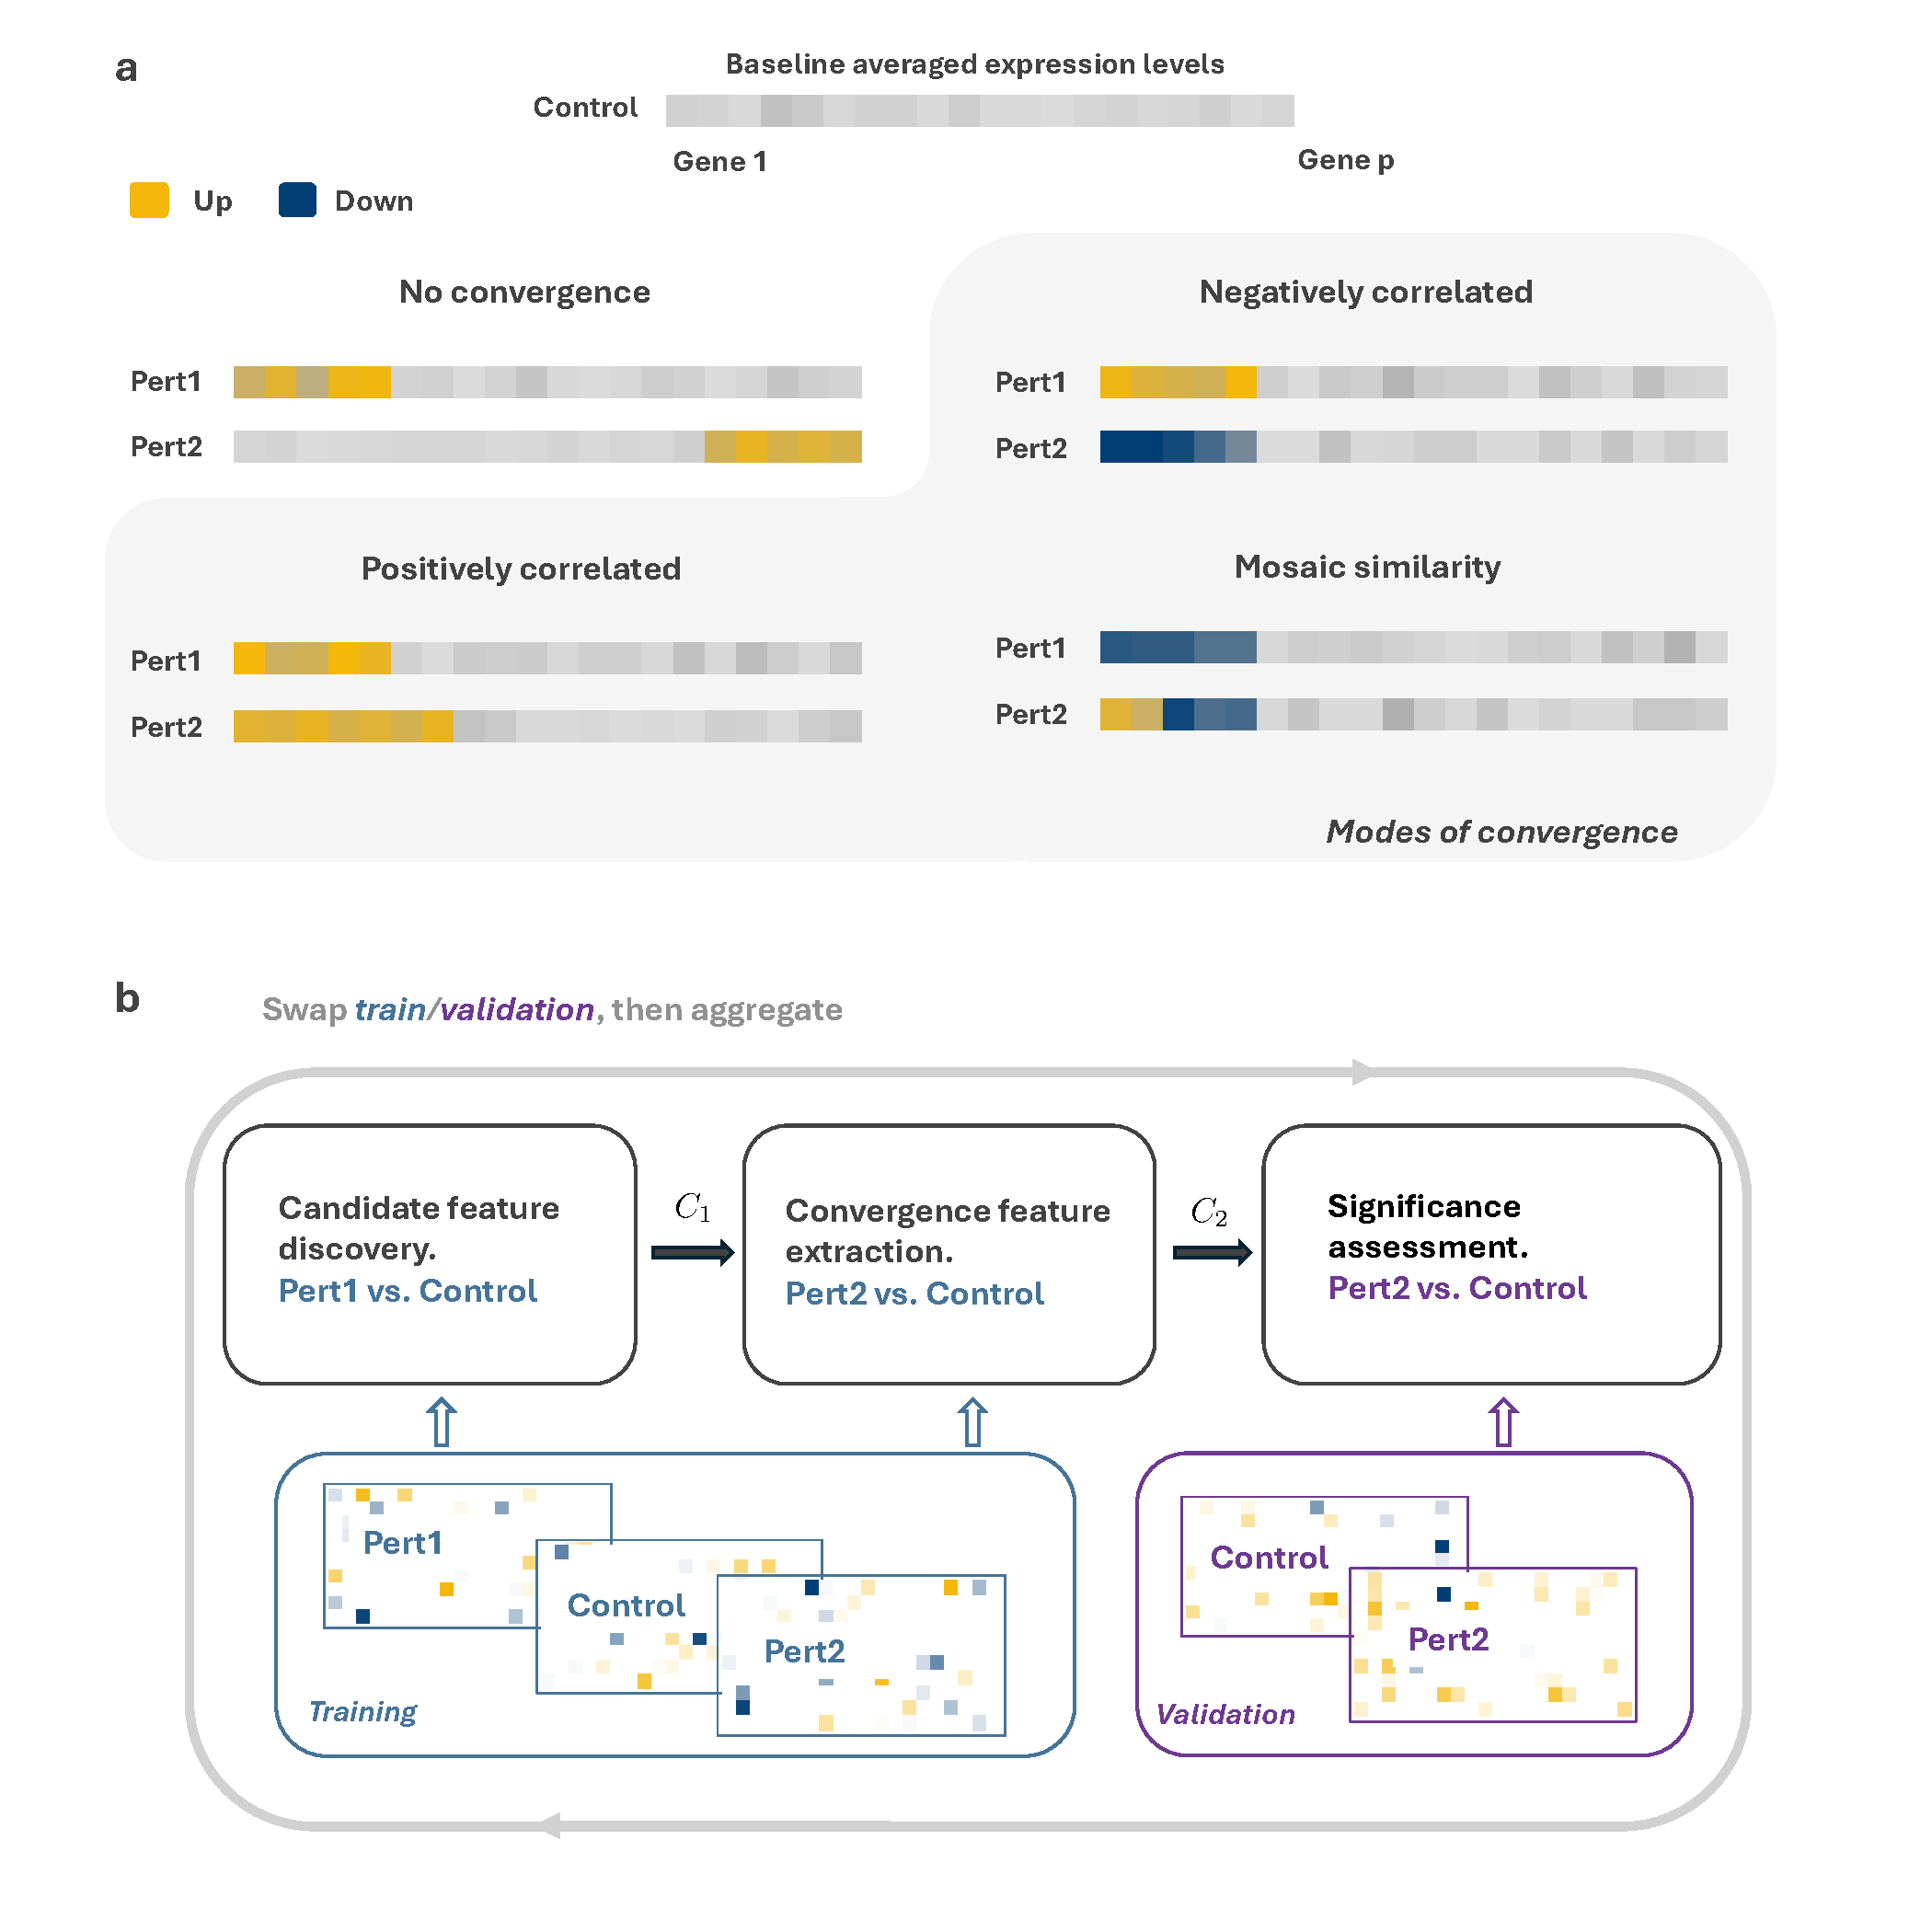
\includegraphics[width=0.8\textwidth]{paper_plot/ppt13_concept_and_flowchart.pdf}
  \caption{\textbf{Genetic convergence and the XConTest pipeline.} \textbf{a} Modes of convergence. We present three patterns of convergence as well as one example where perturbations lead to DE but not convergence. \textbf{b} A diagram of the XConTest pipeline. We use perturbation 1 to discover convergence features (gene or gene modules) and perturbation 2 to validate. }
  \label{fig: concept}
\end{figure}

We model each cell’s expression profile as a high-dimensional random vector, allowing distinct perturbations to induce shifts in average gene expression. Let $\bm{\mu}_c = (\mu_{c1},...,\mu_{cp})$  denote the mean expression levels of $p$ genes in the non-targeting control group. For two perturbation groups, indexed by $K=1,2$, let $\bm{\mu}_K = (\mu_{K1}, \ldots, \mu_{Kp})$ denote the corresponding mean expression profiles. Standard differential expression (DE) analysis asks whether $\bm{\mu}_K = \bm{\mu}_c$ and, if not, which genes contribute to this difference.

Convergence analysis (CA) can be viewed as a second-order analogue of DE analysis. Rather than testing whether a perturbation differs from control, CA asks whether two perturbations induce similar deviations from the control baseline. Defining perturbation-specific effects as $\bm{\Delta}_K = \bm{\mu}_K - \bm{\mu}_c$, CA evaluates the similarity between $\bm{\Delta}_1$ and $\bm{\Delta}_2$. Under our framework, a pair of perturbations is considered convergent when both effect vectors are non-zero and exhibit substantial overlap in their non-zero coordinates.

Such convergence is biologically interpretable as evidence that the perturbed genes participate in related regulatory functions. \Cref{fig: concept}a illustrates several modes of genetic convergence. In the positively correlated setting, both perturbations regulate overlapping downstream pathways in the same direction. In the negatively correlated setting, the downstream targets remain shared, but the regulatory directions are reversed. Importantly, this case should still be classified as convergent, emphasizing that CA is fundamentally distinct from testing the stronger condition $\bm{\Delta}_1 = \bm{\Delta}_2$. We further consider a more general \textit{mosaic} form of convergence, in which perturbations exert heterogeneous effects across overlapping subsets of downstream genes. Formally, two perturbations are mosaic-convergent whenever the supports of $\bm{\Delta}_1$ and $\bm{\Delta}_2$ have a non-empty intersection.

To address this problem, we introduce XConTest, a cross-fitted convergence test for CA settings. The overall workflow is illustrated in \Cref{fig: concept}b. XConTest uses a subset of cells from all three groups (two perturbations and controls) for convergent feature extraction, while reserving held-out cells for inference on the degree of similarity. This sample-splitting strategy mitigates false discoveries arising from feature selection, and embedding it within a cross-fitting framework recovers statistical efficiency by aggregating evidence across multiple splits.

A single pass of XConTest proceeds in three steps. First, using cells from Perturbation 1 and the control group, we train a classifier $\mathcal{C}_1$ on the expression profiles of the $p$ genes to distinguish perturbed from control cells. We use sparse linear classifiers, such as the Lasso \citep{tibshirani1996regression}, so that the fitted model simultaneously performs classification and selects candidate convergence genes from the support of $\bm{\Delta}_1$. Second, we train a second classifier $\mathcal{C}_2$ to distinguish Perturbation 2 from control, restricting the model to genes selected in the first step. In practice, $\mathcal{C}_2$ typically retains only a subset of these genes, corresponding to features that capture the shared signal between $\bm{\Delta}_1$ and $\bm{\Delta}_2$. Third, we apply $\mathcal{C}_2$ to the held-out cells to construct test statistics and calculate p-values for convergence.

Candidate feature extraction can be performed either at the individual-gene level or at the gene-module level. XConTest is modular and can incorporate any upstream method for defining gene programs based on empirical co-regulation patterns, including WGCNA \citep{langfelder2008wgcna}, CS-CORE \citep{su2023cell}, and related approaches \citep{wang2021constructing,schnitzler2024convergence}. In this work, we favor a pipeline combining CS-CORE with WGCNA to identify correlated gene modules prior to convergence testing. In this setting, the features in \Cref{fig: concept} correspond to modules rather than individual genes, and the classifiers $\mathcal{C}_1$ and $\mathcal{C}_2$ are implemented using the Group Lasso \citep{meier2008group} to respect module structure.

This aggregated version of XConTest retains false-discovery control while shifting inference to the biologically meaningful gene-module level. We view this extension as improving both statistical power and interpretability. In particular, when two perturbations affect the same downstream modules without strong gene-level overlap, module-level XConTest can still detect their shared regulatory architecture.

To benchmark XConTest, we also evaluated a Direct Gene Set (Dset) procedure in both simulation studies and real-data examples. Dset is not introduced here as a new methodological contribution; rather, it formalizes a commonly used differential expression (DE)–based practice in the literature. Specifically, it tests whether two perturbations exhibit overlapping DE gene modules. Additional technical details, including family-wise type I error control, are provided in the Materials and Methods section.   This formalization enables a direct assessment of the extent to which XConTest improves upon standard practice.

Although conceptually simple, this Dset benchmark performs well in simulations when only a small number of modules are affected by the perturbations. However, in real Perturb-seq data, where many modules exhibit moderately nonzero effects, it will indicate convergence even when the main signals do not align. In contrast, XConTest better emphasizes the overall profile difference and offers easier interpretation when processing a large number of perturbations. More details will be presented in our case studies.

\subsection*{XConTest controls both type-I and type-II errors}
\label{stat-sim}


\begin{figure}[!tbp]
  \centering  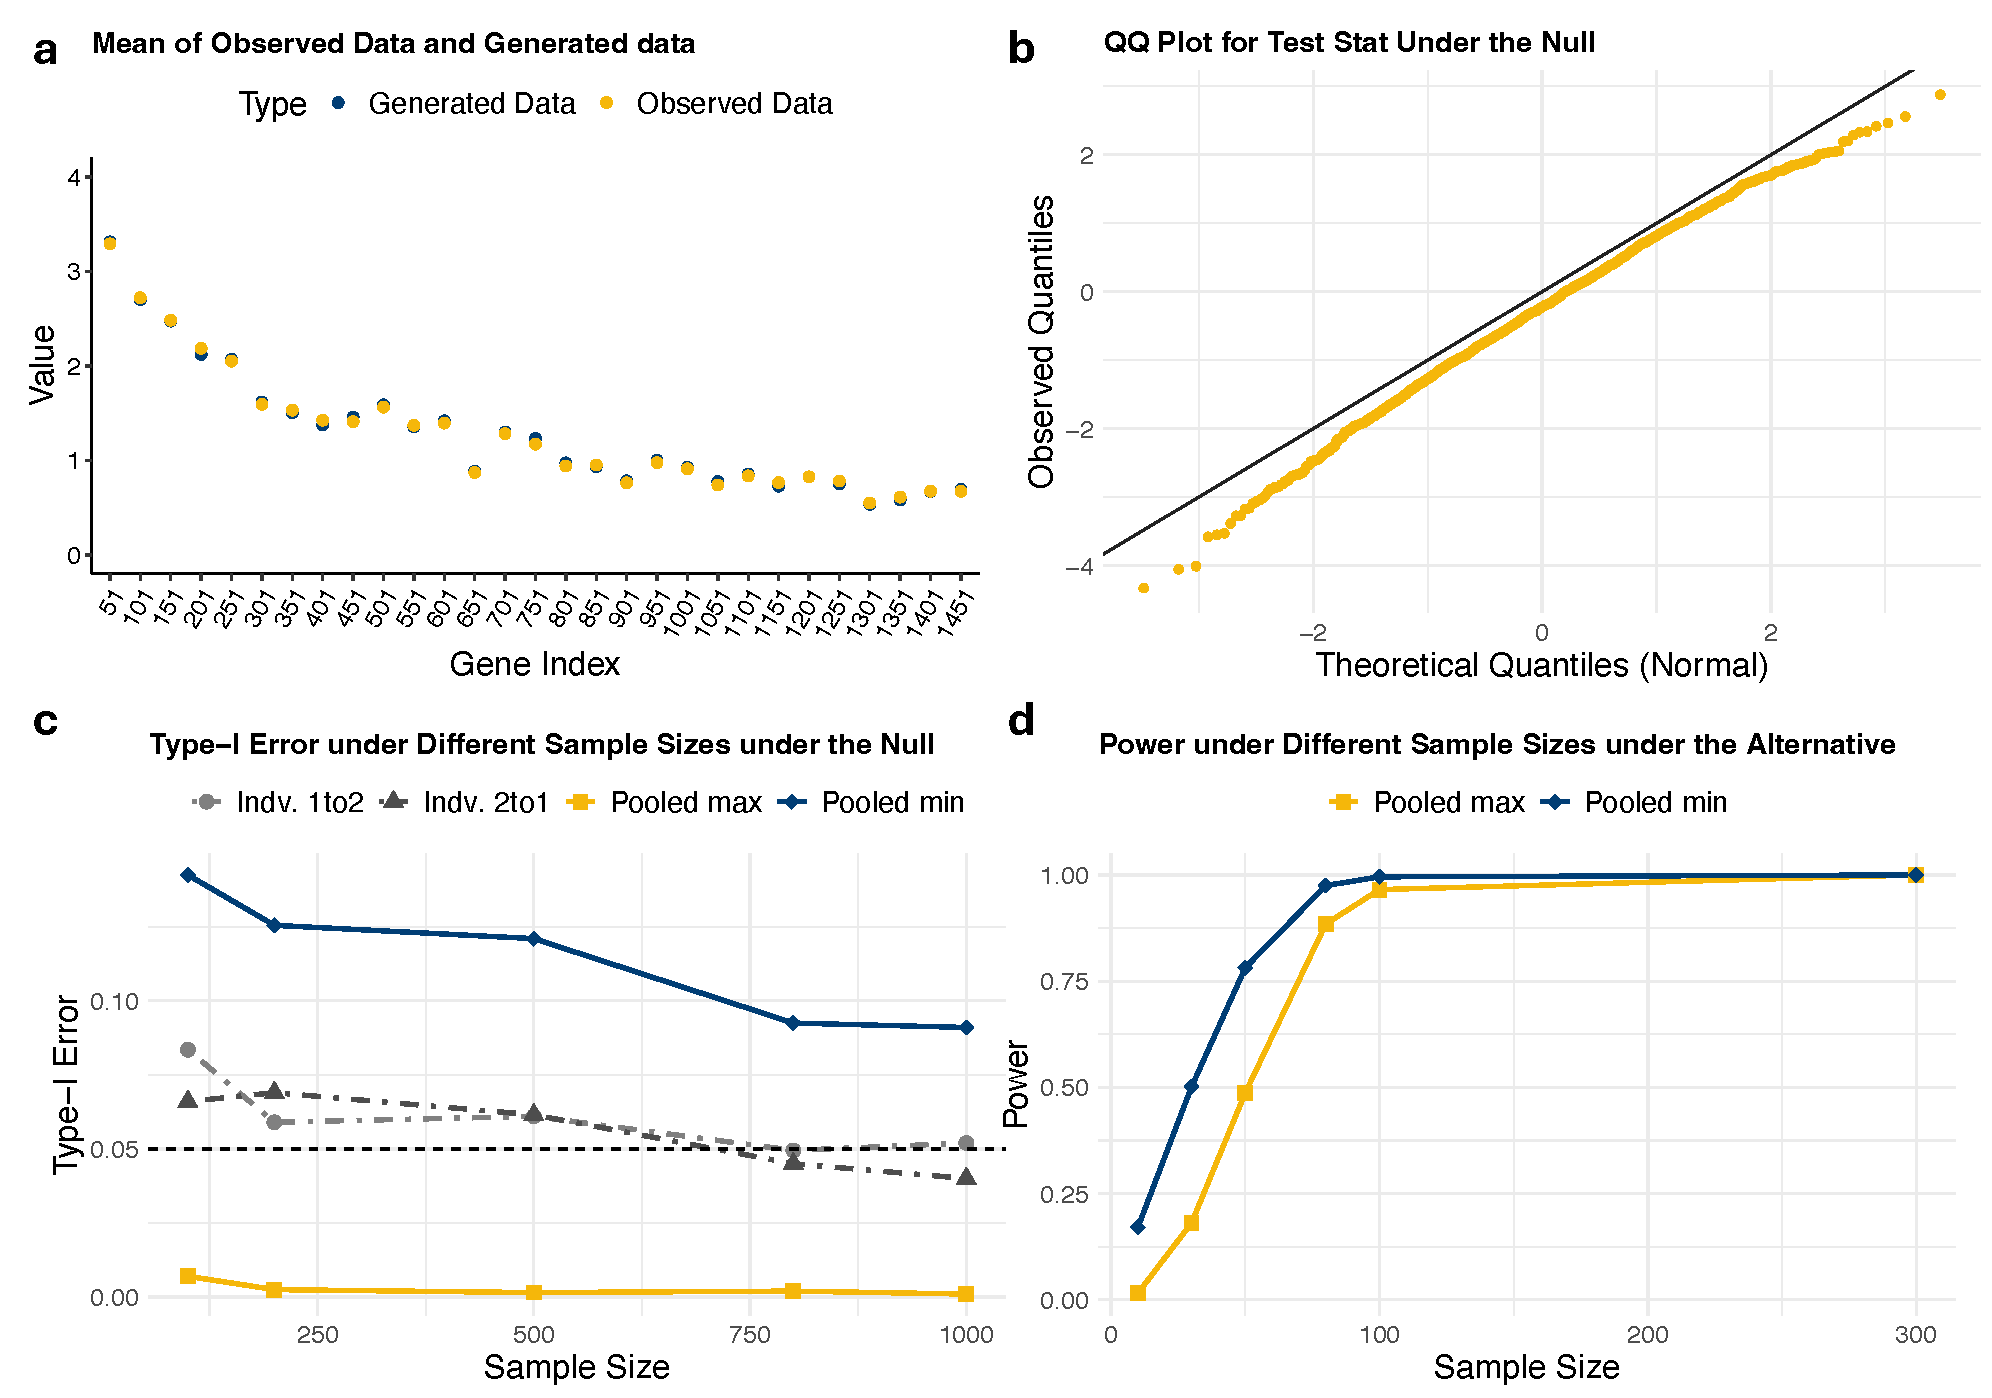
\includegraphics[width=0.9\textwidth]{paper_plot/simulation.pdf}
  \caption{
  \textbf{Simulation Study on XConTest. a.} Mean gene expression of observed and simulated cells. The expression levels overlap well. \textbf{b. }Q-Q (quantile-quantile) plot demonstrates that the test statistic is approximately normal under the null hypothesis. \textbf{c.} Type-I and \textbf{d.}  Power of XConTest under the null and alternative hypotheses. We include results from both individual and pooled p-values. The Pooled max and Pooled min p-values are defined in the main text.}
  \label{fig:sim}
\end{figure}


%A simulation study was conducted to evaluate the statistical performance of XConTest. We use data in \cite{yao2024scalable} to train a generative model that can generate expression profiles of non-targeting cells, and illustrate that the generated cells' expression level matches the original data on a subset of 1,500 highly variable genes (Fig.~\ref{fig:sim}a). A subset of the cells has a subset of genes modified to mimic perturbed groups. To create the null scenario, expression levels of genes numbered \textit{1 to 30} in perturbation group 1 were multiplied by 5, while expression levels of genes numbered \textit{31 to 60} in perturbation group 2 were modified in the same way. Under the alternative scenario, expression levels of genes numbered \textit{1 to 15} in perturbation group 1 were multiplied by 0.95, while expression levels of genes numbered \textit{1 to 5} in perturbation group 2 were multiplied by 0.9.


We evaluated the statistical performance of XConTest through a simulation study. The expression profiles of non-targeting cells were simulated from a diffusion-based generative model \cite{shang2025predicting}, which was trained using the control data from a perturbation experiment \cite{yao2024scalable}. The generated cells' expression levels matched the original data on 1,500 highly variable genes (Fig.~\ref{fig:sim}a). To simulate two perturbation conditions, we modified the expression of a subset of genes in some of the generated cells. The control cells were left unperturbed. 

In the null scenario, expression levels of genes numbered \textit{1 to 30} in perturbation group 1 were multiplied by 5, while expression levels of genes numbered \textit{31 to 60} in perturbation group 2 were modified in the same way. Because the perturbed genes are non-overlapping, there is no convergence despite the five-fold change. Under the alternative scenario, expression levels of genes numbered \textit{1 to 15} in perturbation group 1 were multiplied by 0.95, while expression levels of genes numbered \textit{1 to 5} in perturbation group 2 were multiplied by 0.9. Because the perturbed genes are partially overlapping, there is convergence in this simulation.

The empirical distribution of XConTest's test statistics is compared to the standard normal (sample size = 200, number of genes = 1,500, Fig.~\ref{fig:sim}b). When the sample size is comparable or smaller than the number of measured genes, many statistical procedures do not have easily tractable distributions 
---however, XConTest is designed to have an approximately normal distribution under the null hypothesis, i.e., when there is no convergence.

XConTest is a directional method. When the signal is abundant, the result is insensitive to which perturbation group is used for candidate feature discovery. However, in practical settings, we observe that XConTest may give different inferential results when swapping the roles of the perturbation groups (i.e., when using Pert 2 to construct $\mathcal{C}_1$ in \Cref{fig: concept}b). The asymmetry arises because $\mathcal{C}_1$ captures the most important features for distinguishing the discovery perturbation from the control. This set of genes will inevitably vary when the alternate perturbation group is used to train $\mathcal{C}_1$. We denote the direction presented in \Cref{fig: concept}b as $1\rightarrow 2$ and the reverse direction as $2\rightarrow 1$. These two p-values should both be significant when convergence is established and the sample size is sufficient. However, they are not expected to be numerically identical.
 \Cref{fig:sim}c illustrates that both directions offer well-calibrated testing procedures (with a slight inflation when sample size $<250$). One may consider either $p_{\rm min} = \min(p_{\rm 1to2},p_{\rm 2to1}) < \alpha$ (``Pooled min" in \Cref{fig:sim}c, d) or $p_{\rm max} = \max(p_{\rm 1to2},p_{\rm 2to1}) < \alpha$ (``Pooled max" in \Cref{fig:sim}c, d) as the significance criterion. The former criterion declares convergence when either direction is significant, whereas the latter requires both directions to be predictive. In practice, we recommend using the more stringent criterion based on $p_{\rm max}$ (Fig.~\ref{fig:sim}c). Theoretically, $p_{\rm min}$ can control the overall type-I error at less than $2\alpha$, but in general, it requires an unrealistically large sample size. The maximum criterion offers less power, as expected, but its power reaches one after a moderate number of cells have been collected, even when the convergent genes have only 10\% lower expression than baseline (Fig.~\ref{fig:sim}d). The rest of this paper applies $p_{\rm max} < \alpha$ when reporting significance results. More details on this simulation study are provided in Materials and Methods.

\subsection*{Aggregated XConTest Permits Gene-Module Level Convergence Analysis}\label{artificial-sim}

   
\begin{figure}[tbp]
    \centering
    \includegraphics[width=\linewidth]{paper_plot/06_normalized_convergence_figure.pdf}
    \caption{
    \begin{revblockr3}
    \textbf{Results of aggregated XConTest on simulation data with sparse signals.} \textbf{a.} Average log fold change of gene expression in each gene module. \textbf{b.} Testing results from aggregated XConTest. The upper half shows whether two perturbations are significantly convergent, and the lower half records the number of FSFs (i.e., detected gene modules). 
    \end{revblockr3}}   
    \label{fig: real_data_module_simu}
\end{figure}

\begin{revblockr3}
Measured genes in expression profiles can often be organized into functional modules. Distinct perturbations may affect the same module even when they alter different genes within that module. In this setting, convergence is more naturally defined at the module level rather than at the individual-gene level. To target this form of convergence, we replace the Lasso classifier in XConTest with a group Lasso classifier (Equation~\eqref{eq: group lasso}) so that it can perform module-level feature selection. We refer to the resulting procedure as aggregated XConTest. It identifies two perturbations as convergent when their modified gene modules overlap.

We used a simulation to test whether aggregated XConTest can detect sparse perturbation effects. Based on the non-targting cell data in \cite{shi2026genome}, we created expression profiles for 1,500 genes across six treatment groups and one control group (labeled A--F in \Cref{fig: real_data_module_simu}a, after removing the control baseline). Each perturbed group contained $200$ cells, and the control group contained $400$. The 1,500 genes were partitioned into 30 prespecified modules, and at most five modules were modified for each perturbation. Within each modified module, only approximately 20\% of genes had altered expression levels. Thus, even when two perturbations induce overlapping module-level changes, the specific genes affected within those modules need not coincide. We summarize the simulated perturbation effects using a module-level heatmap, a common visualization in the literature (for example, \cite{schnitzler2024convergence}). The color intensity represents the average log fold change of gene expression within each module (averaged first over samples and then over genes in each module).

We applied aggregated XConTest to the simulated datasets (\Cref{fig: real_data_module_simu}b). The convergence results and the number of Frequently Selected Features (FSFs) are recorded. FSFs are the genes (simple XConTest) or gene modules (aggregated version) that contribute most to the convergence results. Specifically, we define FSFs as features selected in $>50\%$ of the cross-fitting folds. In this experiment, aggregated XConTest shows valid type-I error control. For example, F is not convergent with any other perturbation. Pairs with convergence signals are also successfully identified.

In practice, defining the gene modules is itself a separate modeling step. Modules can be specified using prior biological knowledge, estimated from gene-gene coexpression, or constructed from a combination of both sources. In this simulation, our goal is to assess whether aggregated XConTest can detect convergence when only a small fraction of genes within each module is affected by the perturbations. For this purpose, we provided the true module structure to XConTest to separate convergence testing from module construction. In the real-data analysis reported below, we implement the CS-CORE framework to establish gene modules, which is a reliable method for recovering interpretable modules under moderate signal strength. The Dset method has a similar discovery as XConTest in this conceptual example, while reporting slightly more converged modules (\Cref{Chen_revise_artificial_pert}). However, in real data, it tends to report too many pairs of convergence even though the similarity is minor (e.g., \Cref{fig:yao_2023_main}).


In addition, we conducted a sensitivity analysis using the \textit{Splatter} framework \cite{zappia2017splatter}. In this study, the expression profiles were generated from a carefully designed distribution similar to real-world data, and we further reduced the number of cells. The findings of XConTest are robust to these changes (\Cref{fig: splatter_simulation}).

\end{revblockr3}


% , and a subtle but important distinction between the methods emerged. This distinction can be seen, for example, in the comparison between perturbations A and B (contrasting Figure \ref{fig: real_data_module_simu}b and \Cref{Chen_revise_artificial_pert}). In our simulation setup, all of the first five modules were modified for perturbation B. However, modules 1 and 5 carry only weak signals, which appear as faint blue in \Cref{fig: real_data_module_simu}a. The two methods report different numbers of FSFs for the A--B comparison.
% Dset detects all five modules (1--5) as convergent features. In contrast, XConTest reports only the three modules with substantial signal as its FSFs. This is expected because its sparsity-inducing classifiers exclude modules 1 and 5, which provide little additional predictive capacity once modules 2--4 are included. XConTest avoids reporting modules with weak signals. This behavior is advantageous in real Perturb-seq data, where weak and widespread transcriptional changes are common and may obscure the primary convergence pattern. This distinction is further demonstrated in our Perturb-seq example (\Cref{fig:yao_2023_main}).


\subsection*{Application: CRISPRi Data from a Neuronal Differentiation Study}

Substantial progress has been made in identifying genes associated with autism spectrum disorder (ASD). A key unresolved question, however, is whether these risk genes produce distinct transcriptional programs or converge onto shared downstream molecular mechanisms. To address this, we analyzed the Perturb-seq dataset of \cite{lalli2020high}, in which CRISPR–Cas9–mediated transcriptional repression was coupled with single-cell RNA sequencing to characterize the pathogenic consequences of 13 ASD-associated genes, most of which are supported by multiple independent studies. Because transcriptional programs are expected to be most stable in more differentiated cells, we applied gene-level XConTest to cells from the late pseudotime stage, corresponding to a mature phase of neural differentiation.

The pairwise convergence results for the selected perturbations are summarized in two complementary forms (Fig.~\ref{fig:lalli}a): the upper triangular matrix displays the binary significance calls for convergence, whereas the lower triangular matrix reports the number of overlapping genes in the feature-selected gene sets (FSFs) identified by XConTest for each perturbation pair. This representation highlights both the statistical evidence for convergence and the extent of the shared downstream transcriptional program.

To further evaluate the biological coherence of the detected signal, we performed Gene Ontology (GO) enrichment analysis on the FSF corresponding to the ADNP--PTEN perturbation pair, one of the strongly convergent pairs identified by XConTest. The shared gene set showed pronounced enrichment for pathways related to neural development and neuronal differentiation (Fig.~\ref{fig:lalli}b), supporting the interpretation that these two ASD-associated genes perturb common neurodevelopmental processes.

Taken together, the pairwise convergence map and downstream GO analysis provide strong support for the biological relevance of the detected convergence structure. Beyond identifying statistically significant perturbation pairs, XConTest yields interpretable shared gene sets whose functional enrichment implicates neuronal and synaptic pathways, consistent with the developmental context of the dataset \cite{lalli2020high}. These findings provide orthogonal biological validation of the convergence signals detected by XConTest and further demonstrate its utility for uncovering shared disease mechanisms among ASD risk genes.

\begin{figure}[tbp]
  \centering
  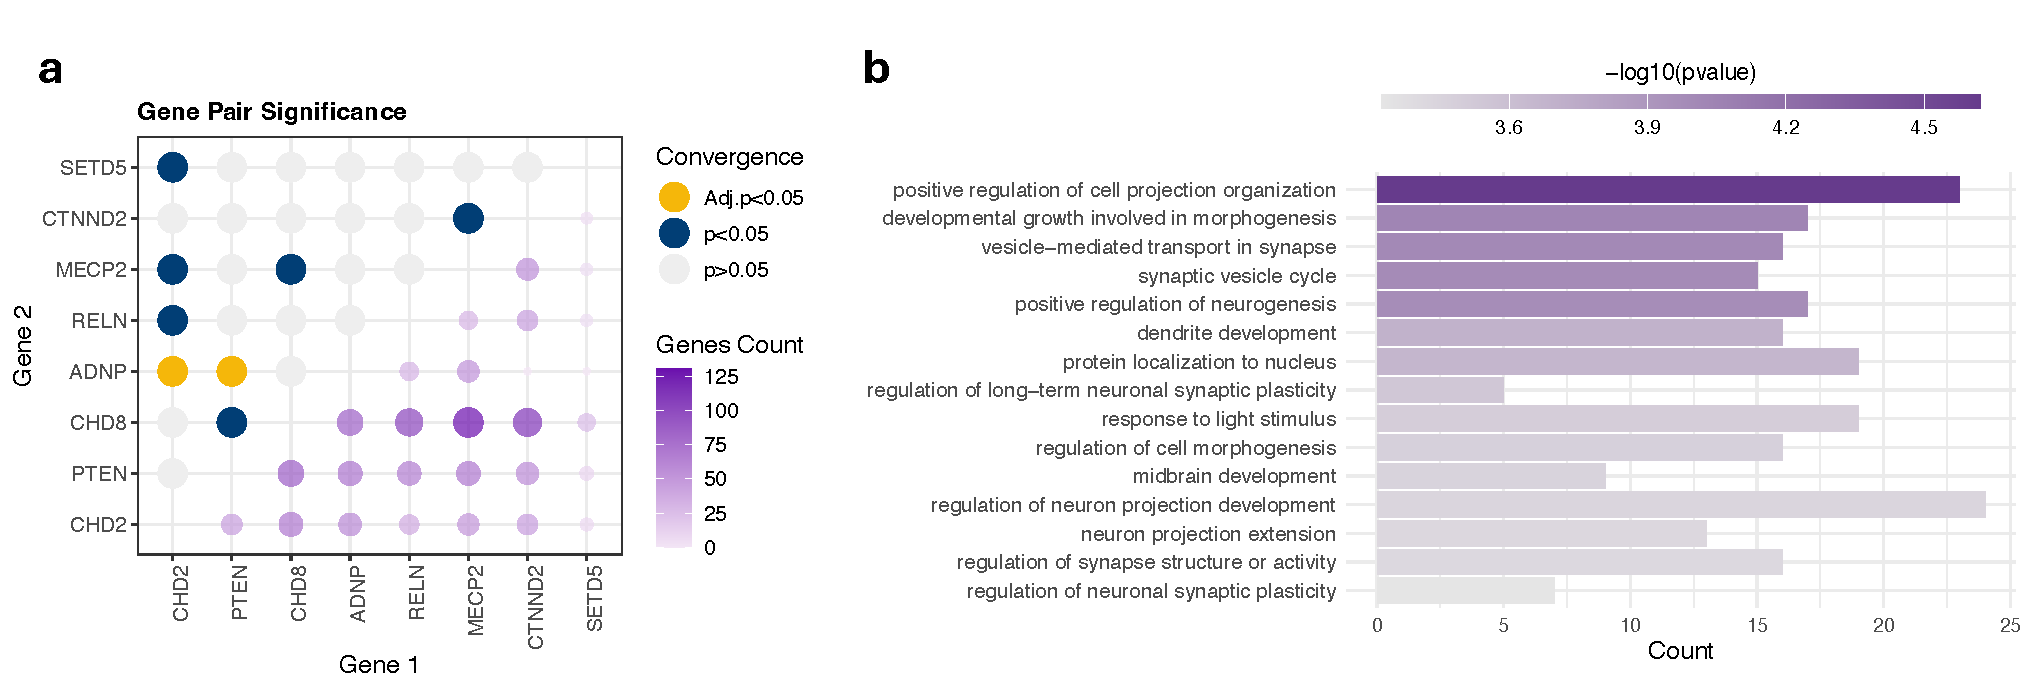
\includegraphics[width=\textwidth]{paper_plot/lalli_conv_and_GO_intersect.pdf}
  \caption{\textbf{Results of Convergence Testing by XConTest on the dataset of \cite{lalli2020high}.} \textbf{a.} shows the binary CA results and number of FSFs for each selected pair \textbf{b.} shows the GO analysis for genes detected where ADNP and PTEN converge. }
  \label{fig:lalli}
\end{figure}

\subsection*{Application: Perturb-seq Profiling of a Human Macrophage Cell Line}

Aggregated XConTest was applied to the data reported in \cite{yao2024scalable} to investigate the functional similarities of 598 genes involved in the immune response to bacterial lipopolysaccharide. Datasets with such a large number of perturbations focused on a narrowly defined biological process are uncommon in the literature. In their study, the authors introduced novel experimental and computational schemes to improve the efficiency of perturbation screening and benchmarked these against standard Perturb-seq. In this investigation, we used the datasets derived from the standard Perturb-seq experiments for simplicity.

The top 50 perturbed genes were selected in \cite{yao2024scalable}, based on their average magnitude of effect on all downstream genes. The genetic convergence results, based on a 2k subset of the total 17k genes, are examined using XConTest (Fig.~\ref{fig:yao_2023_main}a). Among the $1225$ ($50\times 49/2$) unique perturbation pairs, $927$ of them do not yield significant evidence of convergence, when controlling for the type-I error at $0.05$. Among the remaining pairs, $119$ have a strong convergence signal (significant in Bonferroni corrected test).

For comparison, we include the results of Dset in Fig.~\ref{fig:yao_2023_main}b. Recall that this method declares convergence when two perturbations have at least one overlapping differentially expressed gene module. For these data, Dset indicates widespread convergence: $669$ of $1225$ pairs are identified. On the one hand, we carefully adjusted the p-value threshold to control false discoveries and conducted extensive numerical experiments to confirm that Dset is well calibrated when convergence is absent. Thus, we expect that the convergent pairs in \Cref{fig:yao_2023_main}b have at least one overlapping modified module. On the other hand, a small p-value from Dset does not imply that the full expression profiles are substantially similar. Statistical significance may reflect only a minor biological similarity. As a result, Dset reports widespread convergence but provides limited prioritization. The applicability of Dset-like procedures is therefore less clear for conventional Perturb-seq datasets. XConTest uses classifier-based feature selection to filter out weak modules and better prioritize perturbation pairs with more consistent evidence of convergence.


\begin{figure}[!tbp]
  \centering
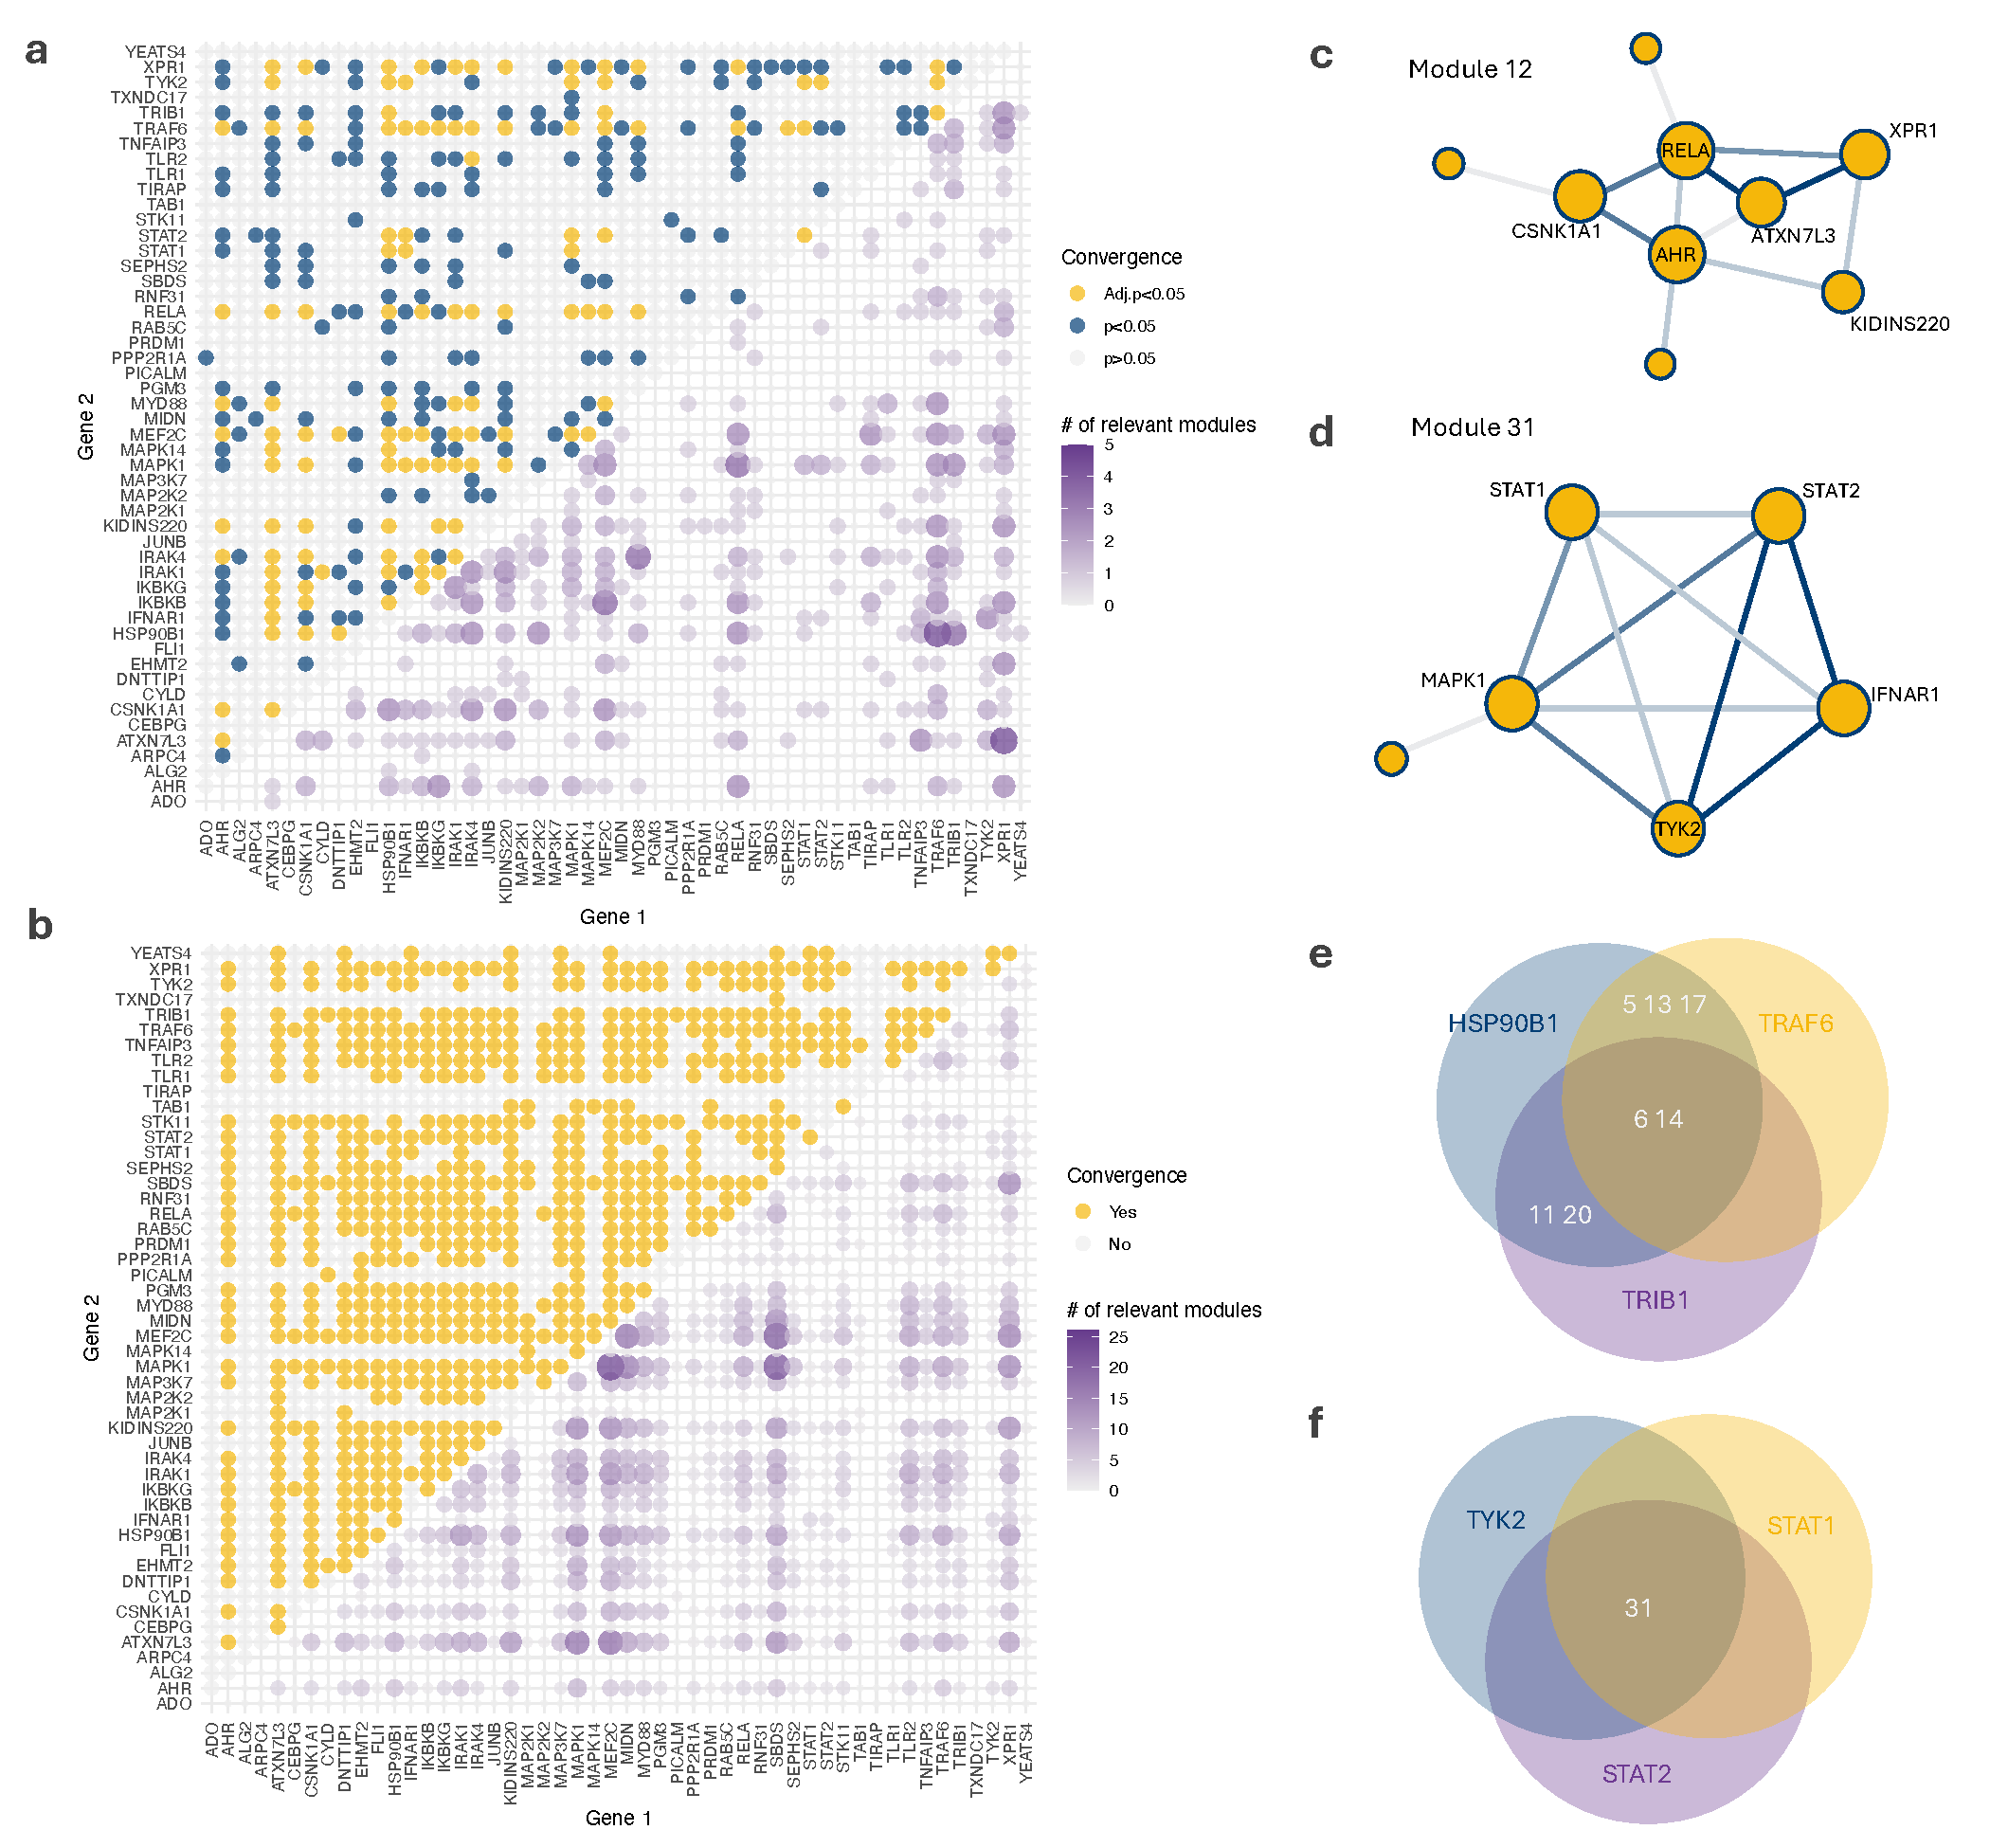
\includegraphics[width=\textwidth]{paper_plot/ppt24_yao_2023.pdf}
  \caption{\textbf{Convergence analysis of the Perturb-seq experiment reported in \cite{yao2024scalable}}. \textbf{a.} Convergence results of aggregated XConTest. The adjusted p-value is the original p-value times the number of perturbation pairs (2450 in this study). \textbf{b.} convergence results of Dset; \textbf{(c–d)} selected gene modules and perturbations that converge on them; \textbf{(e–f)} selected convergent perturbation groups and the modules they converge on. The numbers are module indices. In \textbf{e}, both modules 6 and 14 are selected by all three convergence pairs, but 11 and 20 are unique to the HSP90B1-TRIB1 pair (they converge on 4 modules in total). GO terms of modules frequently appearing in this figure are listed in \Cref{tab: GO of modules Yao 2023}; the complete table is given in \Cref{tab:GO_of_modules_Yao_2023_selected}.  }
  \label{fig:yao_2023_main}
\end{figure}

There are multiple dimensions to further examine the convergence results. Next, we stratify the convergence pairs by active modules (Fig.~\ref{fig:yao_2023_main}c and d). For example, an edge between STAT1 and MAPK1 in panel d indicates that: i) these two perturbations are convergent at $0.05/1225$ type-I error level; and ii) module 31 has been selected as one of the FSFs in both ``STAT1 to MAPK1" and ``MAPK1 to STAT1" directions, which implies a consistent signal. 

\begin{table}[!tbp]
\caption{Representative GO terms associated with selected modules. For each module, we report the biological pathway names with GO IDs. Additional modules are given in \Cref{tab:GO_of_modules_Yao_2023_selected}.}
\vspace{3mm}
\centering
\setlength{\tabcolsep}{12pt} % column separation
\renewcommand{\arraystretch}{1.3} % row spacing
\label{tab: GO of modules Yao 2023}
\begin{tabular}{>{\raggedright\arraybackslash}p{0.15\linewidth} 
                >{\raggedright\arraybackslash}p{0.65\linewidth}}
                
\toprule
\textbf{Module Index} & \textbf{Representative Gene Ontology Terms} \\
\midrule
% 3 & Leukocyte differentiation (0002521); T-helper 17 type immune response (0072538); Lymphocyte activation (0046649)\\
% 5 &  Protein secretion (0009306); Synaptic vesicle endocytosis (0048488)\\
6 & Inflammatory response (0006954); Cytokine production (0001816); Adaptive immune response (0002250)\\
% 11 & Carboxylic acid metabolic process (0019752); Nucleotide metabolic process (0009117)\\
12 & T cell activation (0042110); Lymphocyte activation (0046649); Antigen receptor-mediated signaling pathway (0050851); T cell receptor signaling pathway (0050852)\\
% 13 & Leukocyte migration (0050900); T cell migration (0072678); Leukocyte activation (0045321)\\
14 & Blood vessel development (0001568); Skeletal system development (0001501); Muscle cell differentiation (0042692)\\
% 17 & Inorganic ion homeostasis (0098771); Metal ion transport (0030001)\\
% 18 & Small GTPase-mediated signal transduction (0007264); Actin cytoskeleton organization (0030036)\\
% 20 & Chemotaxis (0006935); Leukocyte migration (0050900); T cell migration (0072678)\\
31 & Response to type I interferon (0034340); Defense response to virus (0051607); Interferon-mediated signaling pathway (0140888); Cytokine production (0001816)\\
\bottomrule
\end{tabular}
\label{GO Table}
\end{table}

We also identified clusters of perturbations that converge on multiple modules (Figs.~\ref{fig:yao_2023_main}e and \ref{fig: convergent greater than 3}), several of which are associated with GO terms relevant to immune-related responses (\Cref{tab: GO of modules Yao 2023}). Three perturbations, HSP90B1, TRAF6, and TRIB1, converge on a larger number of gene modules, suggesting closer functional similarity. All three pairwise comparisons converge on modules 6 and 14. In addition,
HSP90B1 and TRAF6 converge on modules 5, 13, and 17, so this pair converges on five modules in total; HSP90B1 and TRIB1 also converge on modules 11 and 20. Some of the convergent pairs discovered by XConTest align well with prior literature. For example, \cite{wang2024hsp90} provides evidence that Heat Shock Protein 90 (HSP90) contributes to bone destruction in rheumatoid arthritis by promoting osteoclast differentiation through the TRAF6 signaling pathway.

Perturbation clusters that consistently converge on a small number of modules also highlight meaningful functional similarity. For example, perturbations STAT1, STAT2, and TYK2 are pairwise convergent (\Cref{fig:yao_2023_main}f), and module 31, which is strongly related to the response to type I interferon, is the only module selected (\Cref{tab: GO of modules Yao 2023}). All three modified genes are part of the JAK/STAT signaling pathway \citep{rawlings2004jak, hu2021jak}. TYK2, one of the four JAK kinases, participates in phosphorylating membrane cytokine receptors after ligand binding. STAT1 and STAT2 then dock at these sites, are phosphorylated by JAKs, and activate further downstream gene expression. All three genes are well known for their central roles in the type I interferon signaling pathway \citep{velazquez1992protein,qureshi1995tyrosine,prchal2012tyk2}. The convergence results based on current Perturb-seq data support this functional similarity: all three gene pairs show convergence, and only module 31, which is associated with type I interferon, is consistently selected. When examining large-scale convergence results, both broadly convergent pairs and highly specific convergence patterns deserve close attention, as each may point toward important biological mechanisms and opportunities for discovery.

\subsection*{Connecting XConTest Findings with Phenotype and  Pathway Information}


We next compared the XConTest convergence results with phenotype associations reported for the same Perturb-seq data by scLinker \citep{Jagadeesh:2022,yao2024scalable}. scLinker maps GWAS loci for a phenotype to candidate target genes and quantifies the aggregate enrichment of trait-associated signals among genes affected by each perturbation (Supplementary Table 4b in \citealp{yao2024scalable}). For consistency with that analysis, we focused on downstream genes whose expression decreased following knockout, corresponding to positive perturbational effects associated with the targeted gene.

We examined five immune-related phenotypes with strong enrichment in the original study: eosinophil percentage, inflammatory bowel disease (IBD), eczema, rheumatoid arthritis (RA), and primary biliary cirrhosis. Across these phenotypes, XConTest convergence often coincided with phenotype-level convergence from scLinker (Fig.~\ref{fig:four_phenotypes}), supporting the biological relevance of the inferred shared downstream programs. We use the highlighted clusters in Fig.~\ref{fig:yao_2023_main}e and f to illustrate this connection.  

The first cluster includes HSP90B1, TRAF6, and TRIB1, which share module 6 as an FSF (Fig.~\ref{fig:yao_2023_main}e). scLinker also implicated this cluster in eosinophil percentage and RA (Fig.~\ref{fig:four_phenotypes}). The GO terms for module 6 (\Cref{GO Table}) are consistent with eosinophil biology \citep{Fulkerson:2013,Davoine:2014,Jacobsen:2007,Lombardi:2022} and RA immunopathology \citep{mcinnes2011pathogenesis,firestein2003evolving}. This agreement suggests that XConTest captures biologically meaningful downstream convergence, even though there is limited evidence that these genes are direct RA GWAS hits, and only TRIB1 has a strong prior association with eosinophil percentage.

The second cluster includes STAT1, STAT2, and TYK2, which converge on module 31 (Fig.~\ref{fig:yao_2023_main}f). This module is enriched for type I interferon response, antiviral defense, interferon-mediated signaling, and cytokine production (\Cref{GO Table}). scLinker strongly associated STAT1 with IBD, consistent with the role of interferon-driven immune dysregulation in intestinal disease \citep{Tarris:2021,Honap:2024,Giles:2017,Cadwell:2010}. XConTest further suggests that STAT2 and TYK2 may contribute through the same JAK--STAT and type I interferon program; their scLinker GWAS enrichments were borderline significant, supporting a possible disease-relevant shared pathway.

\begin{figure}[!t]
  \centering
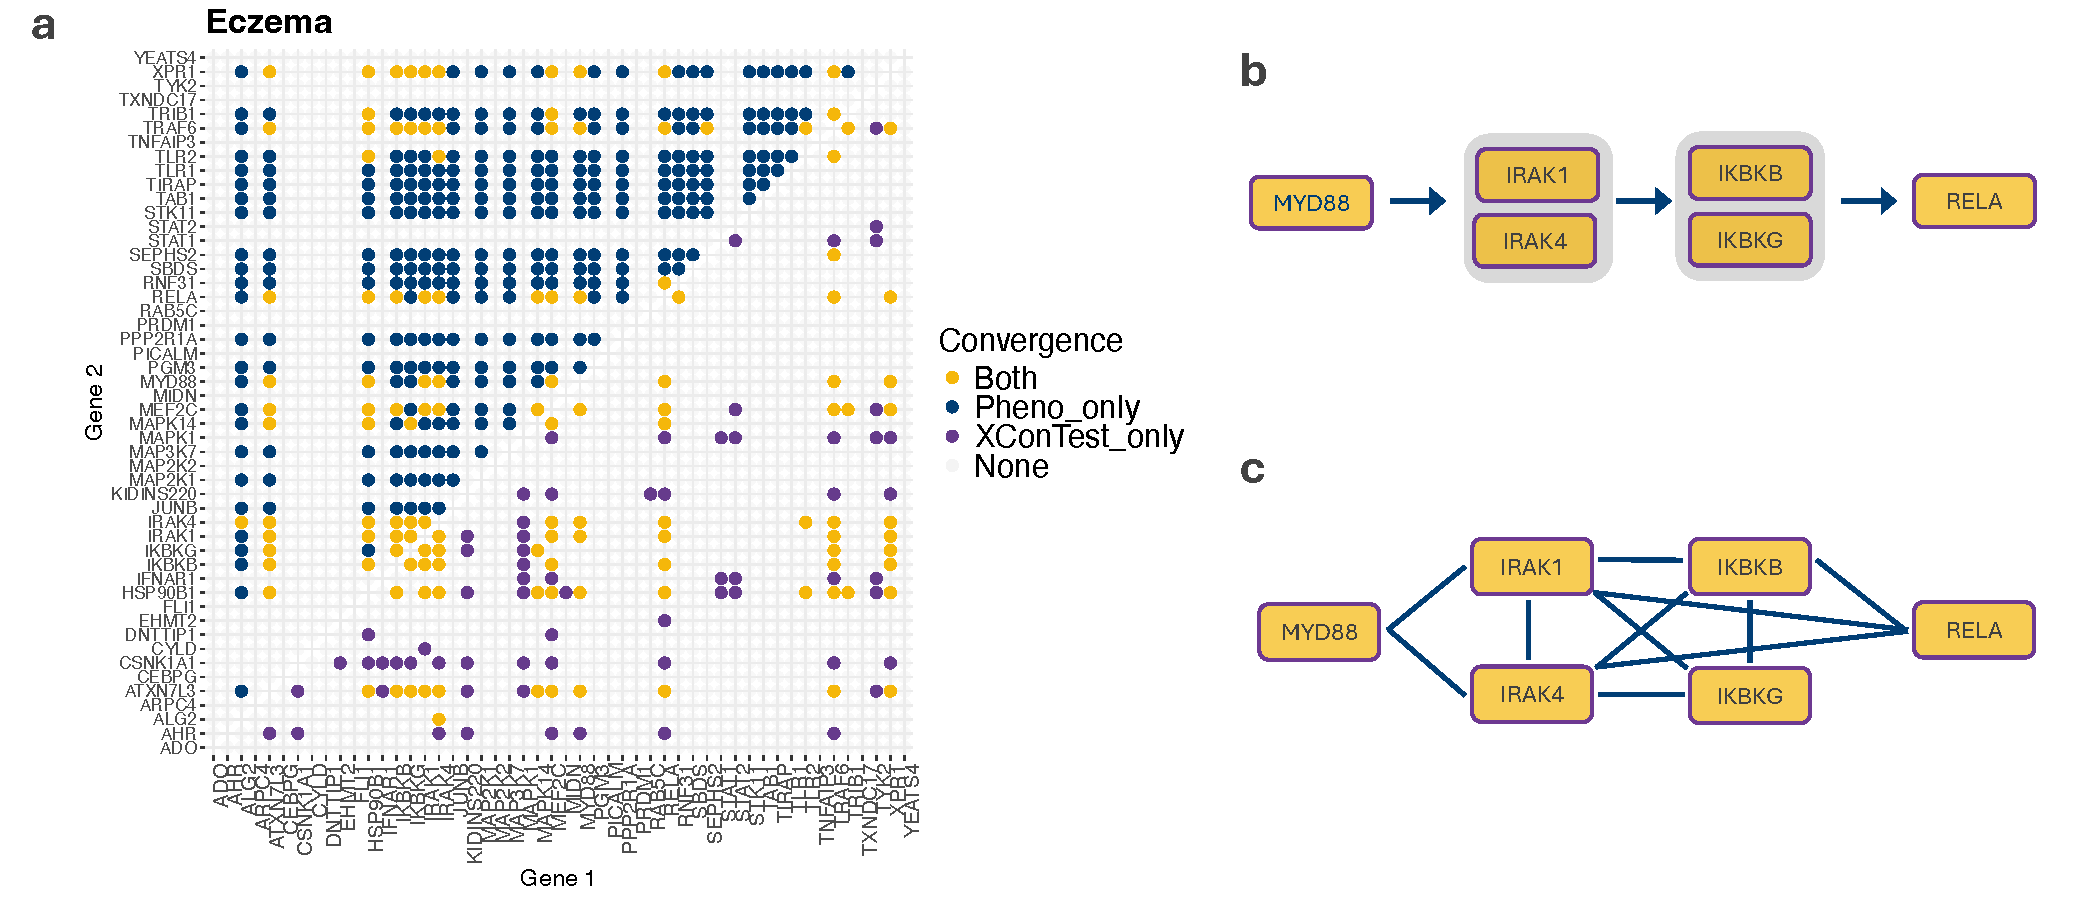
\includegraphics[width=\textwidth]{paper_plot/ppt32_mechanism_and_convergence.pdf}
  \caption{\textbf{Compare XConTest findings with exogenous information. }\textbf{a} Comparison of convergence discoveries by scLinker (upper triangle) and both XConTest and scLinker (lower triangle). \textbf{b} Regulatory ordering of perturbations included in this study within the MYD88-dependent NF-$\kappa$B pathway. \textbf{c} Joint convergence based on scLinker and XConTest closely resembles the mechanism described in \textbf{b}. 
}
  \label{fig:disease_mechanism_convergence}
\end{figure}

In addition, XConTest also recovered convergence patterns aligned with established signaling pathways. Many top convergent pairs mapped to the MyD88-dependent cascade \citep{isnardi2008irak,picard2010clinical,bennett2023paralog}, which links upstream receptor activation to NF-$\kappa$B and MAPK transcriptional programs. For the pathway members shown in \Cref{fig:disease_mechanism_convergence}b, XConTest produced a tightly connected convergence graph (Fig.~\ref{fig:disease_mechanism_convergence}c), while only a small number of outside perturbations showed reproducible convergence with these genes. In contrast, Dset did not recover the same pathway-level specificity (Fig.~\ref{fig:yao_2023_main}b).

Together, these findings support the interpretation that convergent perturbations often reflect shared biological function, especially when they are also supported by phenotype associations or known regulatory circuitry. For example, several MyD88 pathway genes were associated with eczema by scLinker (Fig.~\ref{fig:disease_mechanism_convergence}a). ATXN7L3, which is not currently annotated as a MyD88 pathway component, converged with multiple pathway genes and was likewise associated with eczema, suggesting a possible indirect role in MyD88-mediated inflammatory signaling.

Finally, we compared these findings with parallel analyses based on Dset (Fig.~\ref{fig:DirectscLinker}). Dset identified many convergent pairs, but many likely reflect weaker or less specific associations. Conversely, scLinker detected phenotype-relevant pairs not captured by Dset, indicating that some perturbations can share disease-relevant downstream signals despite limited direct target overlap.

Overall, these results show that convergence analysis can complement GWAS-based interpretation by revealing shared regulatory programs and generating testable hypotheses for genes with unclear disease mechanisms. To assess the robustness of the discovery, we conducted a sensitivity analysis retaining only the expression profiles of immune-related genes (\Cref{fig: sensitivity_analysis}). This restriction excludes perturbation pairs that converge through less relevant biological pathways. Rather than applying aggregated XConTest with the group Lasso, we applied XConTest with a Lasso classifier, a more stringent choice because it requires convergent pairs to induce overlapping signals at the gene level rather than the gene-module level. The most important discoveries in \Cref{fig:yao_2023_main}e,f, and \Cref{fig:disease_mechanism_convergence}c are replicated, including the STAT1-STAT2-TYK2 cluster and the MYD88 pathway.

\section*{Discussion}

Characterizing gene function in human cells has long been a central goal of genomics and systems biology, yet the functions of a substantial proportion of genes remain poorly understood \citep{stoeger2018large}. Recent advances in pooled CRISPR-based perturbation screens with molecular readouts now enable systematic inference of causal gene-regulatory networks. By integrating and iteratively refining insights from such perturbation studies, it is becoming increasingly feasible to delineate causal relationships among genes at scale \citep{rood2024toward}. With XConTest, we address a key aspect of this endeavor---the identification of CRISPR perturbations that exert convergent effects on gene regulation, that is, perturbations influencing a shared set of downstream targets. Unlike heuristic strategies that assess DE heatmaps, such as \Cref{fig: real_data_module_simu}a, XConTest provides a rigorous statistical framework to quantify functional convergence.

For comparison, we illustrate Dset, our formalization of a common DE-based analysis strategy. Dset provides a sensitive but potentially overinclusive means of detecting shared functional outcomes, even when the patterns of perturbation effects differ substantially. In contrast, our XConTest framework employs a sparsity-inducing group Lasso formulation that downweights weak effects across modules. This structure encourages cross-module comparability, such that only perturbations with consistently strong signals are propagated to subsequent inference steps. Consequently, convergence is declared only when strong effects align across perturbations, yielding a conservative yet biologically meaningful measure of functional similarity.


GWAS have identified thousands of human genetic variants associated with various diseases and traits, yet the majority of these variants reside in noncoding regions with unknown target genes and functions. CRISPR-based perturbation experiments now provide a powerful means to interrogate the functional consequences of such variants \citep{morris2023discovery}. \cite{schnitzler2024convergence} introduced an innovative approach that links genetic variants to their putative target genes and leverages Perturb-seq to identify convergent transcriptional effects across perturbations---and, by extension, across variants. XConTest builds on this direction by offering an inferential framework to quantify functional convergence among perturbations. Nevertheless, additional work will be needed to establish an integrated, scalable pipeline for translating these experimental and computational advances into practical applications.

In this study, we focus our analysis on perturbations with scRNA-seq readouts; however, emerging technologies now enable a wide range of multimodal perturbation assays. These include chromatin-based readouts with Perturb-ATAC \citep{adamson2016multiplexed}, protein-level profiling with ProCODE \citep{wroblewska2018protein}, joint RNA–protein measurements with ECCITE-seq \citep{Papalexi2021}, CaRPool-seq \citep{wessels2023efficient} or Perturb-CITE-seq \citep{Frangieh:2021}, as well as combined RNA–chromatin profiling with Perturb-SHARE-seq \citep{otto2023structural}. XConTest is readily extensible to these settings: it can be applied to any high-dimensional or longitudinal outcome data, provided that baseline (control) and perturbation (treatment) groups are clearly defined.

Generative models have been developed to predict the outcome of perturbation experiments that have not been performed \citep{GEARS,scGPT,shang2025predicting}.  \cite{rood2024toward} envision these pseudo-data as one step toward producing a perturbation cell and tissue atlas. Part of attaining that goal would involve including these pseudo-data in the analysis pipeline of XConTest.  This merits further investigation. 

\section*{Resource Availability}
\subsection*{Lead Contact}

Requests for further information and resources should be directed to and will
be fulfilled by the lead contact, Tianyu Zhang (\url{tyz@ucsb.edu}).

\subsection*{Materials availability}
This study did not generate new materials.

\subsection*{Data and code availability}
The \texttt{R} package \texttt{HMC} implementing the XConTest method is freely available at \url{https://github.com/terrytianyuzhang/HMC}. The source code used in our study is deposited at (\url{https://github.com/terrytianyuzhang/genetic_convergence_SA}). Tutorial for implementing XConTest can be found at \url{https://terrytianyuzhang.github.io/HMC/HMC_convergence.html}.

\subsection*{Acknowledgments}
We thank two anonymous reviewers for their helpful comments. We also thank Bernie Devlin for his assistance in contextualizing the findings within the scientific literature. This project was supported by National Institute of Mental Health (NIMH) grant R01MH123184.

\subsection*{Author contributions}
	TZ and KR conceptualized the study; TZ designed the methodology and ES refined the testing procedures.
	TZ and ES created the visualizations; TZ developed the software; All authors contributed to the drafting of the manuscript and discussion of the obtained results. All authors read and approved the final manuscript. 
    KR obtained the funding.

\subsection*{Competing Interests}
The authors declare no competing interests.

\subsection*{STAR Methods}

Detailed methods are provided in the online version of this paper

\subsection*{Supplemental Information}
Supplemental PDF includes: \Cref{Chen_revise_artificial_pert} to \Cref{fig: sensitivity_analysis} and \Cref{tab:GO_of_modules_Yao_2023_selected}.

\bibliographystyle{unsrt}
%\bibliographystyle{apalike}
\bibliography{main}



\newpage

\section*{STAR Methods}

\section*{Key Resources Table}
\begin{table}[!h]
\centering
\begin{tabular}{>{\raggedright\arraybackslash}p{0.30\linewidth}
                >{\raggedright\arraybackslash}p{0.15\linewidth}
                >{\raggedright\arraybackslash}p{0.45\linewidth}}
\toprule
\textbf{REAGENT or RESOURCE} & \textbf{SOURCE} & \textbf{IDENTIFIER} \\
\midrule
Dataset & & \\
\midrule
CROP-seq neuronal differentiation & GEO \citep{lalli2020high} & GSE142078 \\
Perturb-seq THP-1 cell line, conventional KO screen & GEO \citep{yao2024scalable} & GSE221321, subset GSM6858447\\ 
& & \url{https://www-ncbi-nlm-nih-gov.proxy.library.ucsb.edu/geo/query/acc.cgi?acc=GSE221321} \\
\midrule
Software and algorithms & & \\
\midrule
XConTest implemented in R package HMC  & This manuscript & \url{https://terrytianyuzhang.github.io/HMC/HMC_convergence.html} \\
CS-CORE & \cite{su2023cell} & \url{https://changsubiostats.github.io/CS-CORE/articles/CSCORE.html} \\
WGCNA & \cite{langfelder2008wgcna} &   \url{https://fuzzyatelin.github.io/bioanth-stats/module-F21-Group1/module-F21-Group1.html} \\
grpreg & \cite{breheny2015group}  & \url{https://pbreheny.github.io/grpreg/} \\
\bottomrule
\end{tabular}
\end{table}

\section*{Method Details}
\subsection*{Data Acquisition}

We evaluated our methods using two genome-scale CRISPR datasets. The Neuronal Differentiation Study targets 14 neurodevelopmental genes, including 13 autism risk genes, in LUHMES human neural progenitor cells \citep{lalli2020high}. After CRISPR targeting, cells were differentiated into postmitotic neurons and their transcriptomes were profiled using droplet-based scRNA-seq \citep{zheng2017massively}. The data related to this work was downloaded from NCBI Gene Expression Omnibus (GEO; \url{https://www.ncbi.nlm.nih.gov/geo/}) under accession number GSE142078. We implemented the preprocessing scripts provided in the supplementary materials of \cite{lalli2020high}.

The Human Macrophage Cell Line dataset assesses the impact of 598 genes in the immune response to bacterial lipopolysaccharide \citep{yao2024scalable}. The study investigated the performance of two experimental knock-out procedures, but we restricted our analysis to data derived from conventional perturb-seq methods. The related data was downloaded from GEO GSE221321. 

\subsection*{Data Processing}

In the analysis of data from \cite{yao2024scalable}, we started from the raw UMI count matrix. We first restricted the analysis to the 2,000 genes with the highest average expression among non-targeting control cells and removed low-quality cells using standard quality-control filters: more than 500 detected genes, fewer than 20k total RNA counts, and less than $10 \%$ mitochondrial reads. We then adjusted each gene separately using a Poisson regression model. Formally, for gene $g$, we modeled the count $Y_{g}$ as Poisson with $\log \mu_{g}=\alpha_g+\beta_{g, 1} I\left({\mathrm{G} 2 \mathrm{M}}\right)+\beta_{g, 2} I\left(\mathrm{S}\right)+\log (\text{library size})$, where $\alpha_g$ is a gene-specific intercept, $I(\cdot)$ is an indicator for cell-cycle state, and $\mu_{g}$ is the expected count of $Y_{g}$. We then formed an adjusted expression value by removing the estimated cell-cycle effect and normalizing by the total RNA count, so downstream analyses were carried out on this residualized, depth-normalized expression matrix rather than on raw counts. No additional feature-wise standardization is required to implement the convergence tests. Log transformations of gene expression, as well as most batch-effect removal procedures, are also compatible with the XConTest framework.

\subsection*{The XConTest Method}

XConTest partitions the data into multiple folds, using a subset of the samples to identify potentially convergent genes and reserving the remaining samples to quantify the signal strength. In practice, the number of folds, denoted by \texttt{NumFold}, is typically set between 5 and 10 to balance estimation quality and computational efficiency.

Below, we provide further details on the proposed XConTest framework. More intuition and explanation are given afterwards.

(1) We collect transcriptomic profile data from the control, perturbation 1, and perturbation 2 groups, withholding a $(\texttt{NumFold})^{-1}$ proportion of samples from each group for subsequent significance assessment. This held-out data is referred to as the validation data.

(2) In the training step, we have three collections of single-cell profiles: $\mathcal{D}_{\texttt{p1}}$, $\mathcal{D}_{\texttt{p2}}$, and $\mathcal{D}_{\texttt{con}}$, corresponding to the Perturbation 1, Perturbation 2, and Control groups, respectively. Each cell is represented by an expression vector $\bm{X}=(X_1,\ldots,X_p)^{\top}\in\mathbb{R}^p$, where $p$ denotes the number of genes. When pooling any two of these datasets, the combined samples can be treated as random draws from a mixture distribution of two populations.

(3) We append a categorical group label $Y\in\{\texttt{con}, \texttt{p1}, \texttt{p2}\}$ to each $\bm{X}$. We first fit a logistic Lasso model regressing $Y$ on $\bm{X}$ using $\mathcal{D}_{\texttt{con}}$ and $\mathcal{D}_{\texttt{p1}}$:
\begin{equation}\label{eq: C1 beta}
   \widehat{\bm \beta}_1 = \arg\min_{\bm{\beta}\in\mathbb{R}^p} \sum_{i} \texttt{logit-loss}(Y_i, X_i^\top \bm{\beta}) + \lambda \|\bm{\beta}\|_1 
\end{equation}
where the summation is over all samples $i\in \mathcal{D}_{\texttt{con}}\cup\mathcal{D}_{\texttt{p1}}$. The sparse regression coefficients $\widehat{\bm \beta}_1$ implies the classifier $\mathcal{C}_1$ in \Cref{fig: concept}b. We denote the support of $\widehat{\bm{\beta}}_1$, that is, the set of genes with non-zero estimated coefficients, by $s_1 \subset \{1,\ldots,p\}$. The hyperparameter $\lambda$ of Lasso is determined using a further nested cross-validation within $\mathcal D_{\texttt{con}}$ and $\mathcal D_{\texttt{p1}}$.

(4) Fit another logistic Lasso model, regressing $Y$ on $\bm{X}$ using $\mathcal{D}_{\texttt{con}}$ and $\mathcal{D}_{\texttt{p2}}$. The coefficients are denoted as $\widehat{\bm \beta}_2$ and its formula is almost identical to that of $\widehat{\bm \beta}_1$: but it is restricted to have zero in all dimensions outside $s_1$. The coefficients $\widehat{\bm{\beta}}_2$ defines the classifier $\mathcal{C}_2$ in \Cref{fig: concept}b. 

% We denote the support of $\widehat{\bm \beta}_2$ as $s_2$: by construction $s_1\subset s_2$. 

Compute the leading Principal Component (PC1), $\hat{\bm{v}}$, using $\mathcal{D}_{\texttt{con}}$. Similarly, we only allow genes in $s_1$ to have non-zero loadings.

In practice, the constraints on $\widehat{\bm{\beta}}_2$ and $\hat{\bm{v}}$ are readily implemented by trimming dimensions outside $s_1$, applying standard software for logistic regression or PCA, and padding zeros to recover the full $p$-dimensional vectors.

(5) Define the CA projection direction as (normalized to have a unit Euclidean norm):
$$
\widehat{\bm{\beta}}_{\texttt{proj}} = \hat{\bm{v}} + w_n\widehat{\bm{\beta}}_{2}.
$$
where $w_n$ is a weighting parameter that diverges with increasing sample size. In this study, we set $w_n = (2n)^{1/3}$, where $n$ denotes the smallest sample size among $\mathcal{D}_{\texttt{p1}}$, $\mathcal{D}_{\texttt{p2}}$, and $\mathcal{D}_{\texttt{con}}$.

(6) Let $\widehat{\bm{\Delta}}_2$ denote the estimated sample mean difference between the perturbation 2 and the control groups. We project this estimated difference onto $\widehat{\bm{\beta}}_{\texttt{proj}}$ to obtain
$$
T_{\texttt{split-1}} = \widehat{\bm{\Delta}}_2^\top \widehat{\bm{\beta}}_{\texttt{proj}}.
$$
The corresponding standard error is estimated as
$$
\hat\sigma_{\texttt{split-1}} = \sqrt{\frac{\texttt{NumFold}}{n_c}\widehat{\operatorname{Var}}_c(\bm{X}^\top \widehat{\bm{\beta}}_{\texttt{proj}}) + \frac{\texttt{NumFold}}{n_2}\widehat{\operatorname{Var}}_2(\bm{X}^\top \widehat{\bm{\beta}}_{\texttt{proj}})}
$$
where $n_c, n_2$ are the total sample sizes from control and perturbation 2. The operator $\widehat{\operatorname{Var}}_c(\cdot)$ represents the sample variance of the projection scores computed using control cells in the validation set, and $\widehat{\operatorname{Var}}_2(\cdot)$ is defined analogously for the perturbation 2 cells.

(7) Finally, we repeat steps (1)–(6) across all cross-validation folds to obtain fold-specific test statistics $T_{\texttt{split-}j}$, $j = 1,\ldots,\texttt{NumFold}$. The overall test statistic is computed as
$$
T = (\texttt{NumFold})^{-1}\sum_{j=1}^{\texttt{NumFold}} T_{\texttt{split-}j}.
$$
Its standard error is estimated by
$$
\hat\sigma = (\texttt{NumFold})^{-2}\sum_{j=1}^{\texttt{NumFold}} \hat\sigma_{\texttt{split-}j}.
$$

\subsection*{Intuition and properties of XConTest}


In equation \eqref{eq: C1 beta}, we use logistic regression to extract features that effectively distinguish perturbation 1 from the control. In step (4), we then train another classifier, $\hat{\bm \beta}_2$, using only the genes selected by $\widehat{\bm{\beta}}_1$. If the two perturbations are truly convergent---that is, if they share a non-negligible signal on a common subset of genes relative to the control---then $\hat{\bm \beta}_2$ will typically remain non-zero and will still help distinguish perturbation 2 from the control.

The projection direction $\widehat{\boldsymbol{\beta}}_{\text {proj }}$ is defined as a linear combination of the leading PC direction and the classifier direction. Since $w_n = (2n)^{1/3}$, $\widehat{\boldsymbol{\beta}}_{\text {proj }}$ is well aligned with $\widehat{\boldsymbol{\beta}}_2$ when $\widehat{\boldsymbol{\beta}}_2$ is non-zero and the sample size is moderately large ($(2\cdot 100)^{1/3} = 5.8$). In that regime, the projection $\widehat{\boldsymbol{\beta}}_{\text {proj }}$ inherits much of the discriminating power of $\widehat{\boldsymbol{\beta}}_2$.

However, we do not set the projection direction equal to $\widehat{\boldsymbol{\beta}}_2$ directly, because sparse-inducing methods may return the zero vector when the shared signal is weak. A natural fallback is the leading PC direction, which may still capture a general trend in the candidate convergence genes. The linear combination in step (5) is designed to interpolate between these two regimes: when the shared signal is strong, the method leans toward $\widehat{\boldsymbol{\beta}}_2$ to improve power; when the shared signal is weak, the PC direction stabilizes the procedure. In particular, because the leading PC is rarely degenerate, this construction helps produce a regular test statistic even when the perturbations do not converge.

Steps (6)--(7) evaluate this learned direction on the held-out data to quantify the degree of convergence.

The resulting studentized statistic, $T / \hat{\sigma}$, is approximately standard normal under mild regularity conditions. A formal theoretical justification is provided in Corollary 3.2 of \cite{zhang2024adaptive}. Notably, while many high-dimensional statistics deviate from normality asymptotically, the test statistic in our framework retains a Gaussian limiting distribution.

A smaller $w_n$ diminishes the impact of $\widehat{\boldsymbol{\beta}}_2$, which reduces power. At the same time, we need $w_n$ to be no larger than $n^{1/2}$ to establish asymptotic normality. The current choice balances these two considerations.


\subsection*{Aggregated XConTest}

We recommend conducting CA on the gene-module level as demonstrated with the data from \cite{yao2024scalable}. The pipeline is very similar to that of gene-wise XConTest. The aggregated XConTest has one extra preprocessing step:

(pre) Divide the $p$ genes into gene-modules using any available methods. We implemented the pipeline that integrates CS-CORE and WGCNA (a vignette is available at \url{https://changsubiostats.github.io/CS-CORE/articles/CSCORE.html}). For genes not strongly associated with any others, we further divide them into smaller modules based on their GO similarity.

The only modified steps are Step (3) (See Equation \Cref{eq: C1 beta}) and Step (4) (the Step right below Equation \ref{eq: C1 beta}). Instead of fitting a logistic Lasso, we need to incorporate the grouping information and solve the group Lasso optimization:
\begin{equation}\label{eq: group lasso}
   \widehat{\bm \beta} = \arg\min_{\bm{\beta}\in\mathbb{R}^p} \sum_{i} \texttt{logit-loss}(Y_i, X_i^\top \bm{\beta}) + \lambda \sum_{j=1}^k \sqrt{\left|G_j\right|} \cdot \|\bm{\beta}_{G_j}\|,
\end{equation}
where $k$ is the number of gene modules, $|G_j|$ is the number of genes in the $j$-th module and $\|\bm{\beta}_{G_j}\|$ is the norm of $\bm{\beta}$ restricted on group $j$ only. We applied the \texttt{cv.grpreg()} function in R package \texttt{grpreg} \cite{breheny2015group} to fit the group Lasso \eqref{eq: group lasso}. The set $s_1$ in step (3) are all the genes in the selected modules of $\widehat{\bm{\beta}}_1$.

\subsection*{The Dset method}\label{app: p-value direct method}

In this section, we describe the Dset benchmark used for comparison with XConTest in several examples. Dset is intended as our formalization of a common literature practice rather than as a new methodological contribution. A pairwise Dset comparison consists of three steps:

(1) Divide the full list of genes into modules. We will implement CS-SCORE in this step as well, for the ease of comparison to XConTest. This step would be idetical to the (pre) step of aggregated XConTest.

(2) Apply a DE test to each of the established modules. In this work, we considered the powerful test introduced in \cite{10.1214/09-AOS716}.

(3) If both Perturbation 1 and 2 establish a significant DE signal on the same module, we claim that they are convergent. The significance level needs to be carefully adjusted to control familywise type-I error, detailed below.

Let $N$ denote the number of perturbations under comparison. And let $M$ be the number of gene modules established in step (1).

\begin{equation*}
    \begin{aligned}
        & \text{Prob}(\text{Dset reports at least one pair converge} \mid H_0) \\
        & \leq \sum_{1\leq i<j\leq N}\text{Prob}(\text{Dset reports perturbations $i$ and $j$ converge} \mid H_0)\\
        &  = \sum_{1\leq i<j\leq N} \text{Prob}(\text{At least one module reported to be DE for both $i$ and $j$} \mid H_0) \\
        & \leq \sum_{1\leq i<j\leq N} \sum_{k=1}^M \text{Prob}(\text{$i$ and $j$ are both DE on module $k$} \mid H_0) \\
        &\leq \sum_{1\leq i<j\leq N} \sum_{k=1}^M \text{Prob}(\text{$i$ is DE on module $k$} \mid H_0) \\
        &\leq \binom{N}{2} \cdot M \cdot p
    \end{aligned}
\end{equation*}

To control the family-wise type-I error at level $\alpha$, we need to set the significance level of each DE test at no larger than $\alpha\binom{N}{2}^{-1} M^{-1}$. In the artificial perturbation setting (\Cref{fig: real_data_module_simu}), $M=30$, $N=6$.

\subsection*{Simulating data via diffusion models}

A simulation study was conducted to evaluate XConTest under the null and alternative hypotheses. The data were simulated from a diffusion-based model \cite{shang2025predicting}, which was trained using the perturbation experiment reported in \cite{yao2024scalable}.

Many methods have been developed to simulate single-cell profiles, including approaches such as \cite{cao2021benchmark} that primarily rely on Poisson or negative binomial assumptions. More recently, deep generative models have become important tools for simulating single-cell profiles that closely resemble the training data. Among these models, diffusion models have advanced rapidly and now represent the state of the art. Examples include \textit{scDiffusion} \citep{10.1093/bioinformatics/btae518}, \textit{cfDiffusion} \citep{10.1093/bib/bbaf071} and \textit{dbDiffusion} \cite{shang2025predicting}. The simulated data in \Cref{fig:sim} were produced using dbDiffusion.

dbDiffusion was inspired by cfDiffusion \citep{10.1093/bib/bbaf071}, which conditions the score function on a one-hot encoding of the category label $c$ (e.g., cell type or perturbation condition). Instead of using the one-hot encoding, dbDiffusion represents each cell type using a low-dimensional embedding derived from principal component analysis (PCA). This embedding captures similarities among cell types while substantially reducing the dimensionality of the conditioning space. The resulting reduction in model complexity yields a more stable estimation procedure and has been shown to produce improved predictions \cite{shang2025predicting}. The generated non-targeting cells had gene-expression profiles that were highly similar to those of the observed non-targeting cells (\Cref{fig:sim}a).


% We used the mean of the embeddings across all treatment cell types as the embedding for non-targeting cells. 

% Afterward, to create the null scenario, expression levels of genes numbered \textit{1 to 30} in perturbation group 1 were multiplied by 5, while expression levels of genes numbered \textit{31 to 60} in perturbation group 2 were modified in the same way. While they are both different from the control, the modified genes do not overlap, so this pair does not converge.

% Under the alternative scenario, expression levels of genes numbered \textit{1 to 15} in perturbation group 1 were multiplied by 0.95, while expression levels of genes numbered \textit{1 to 5} in perturbation group 2 were multiplied by 0.9.


\subsection*{Type-I error and power assessment}

To test the approximate normality of the test statistic under the null hypothesis (no convergence), we generated cell expression profiles using the diffusion model discussed above (repeated 2000 rounds). The generated cells are divided into three groups, each containing 200 samples: a non-targeting group, a perturbation 1 group in which genes indexed 1–30 are up-regulated fivefold, and a perturbation 2 group in which genes indexed 31–60 are up-regulated fivefold. While they are both different from the control, the modified genes do not overlap, so this pair does not converge.
The distribution of the 2000 test statistics was examined in \Cref{fig:sim}b. Specifically, we illustrated the test statistics obtained by experiment $1\rightarrow2$, where the perturbation 1 group is used for candidate feature discovery and perturbation 2 for validation.
 
The simulation setting in \Cref{fig:sim}c is the same as the one in \Cref{fig:sim}b, where we only varied the sample sizes. When calculating the Type-I error, we accounted for the directional nature of our method and compared several approaches for pooling p-values, including $p_{\rm min}$ and $p_{\rm max}$ as defined in the main text. 

The power of XConTest was evaluated under different sample sizes. To simulate convergent perturbations, we perturbed genes indexed by 1–15 by a factor of 0.95 in the perturbation 1 group, and genes 1–5 by a factor of 0.9 in the perturbation 2 group. Results are shown in \Cref{fig:sim}d.

When the number of perturbation pairs is large, as in the case study in \cite{yao2024scalable}, it is essential to employ adjusted p-values to control for the family-wise error rate (or the false discovery rate).

\subsection*{Simulation with perturbed gene modules}

\begin{revblockr3}
We utilized real perturb-seq data to simulate the data for this experiment.  The data are from a published study involving in vivo perturbations in mouse brain \cite{shi2026genome}. This dataset contains many different brain cell types and more than 1000 perturbations. We chose the nontargeting cells in the thalamic glutamatergic neurons (labeled as Prkcd Grin2c Glut) for the current study.

Our numerical experiment induces signals (i.e., mean shifts) among the top 1500 expressed genes. Then, we randomly sampled (without replacement) $400+200\times6=1600$ cells from all non-targeting cells and divided them into one control group (containing 400 cells) and 6 treatment groups (200 cells each); they were labeled A-F in \Cref{fig: real_data_module_simu}a.

In group A, modules 1-5 are up-regulated by factors ranging from 1.3 to 1.5. In group B, modules 1-5 are down-regulated by factors ranging from 0.5 to 0.95. In group C, modules 6-10 are up-regulated by factors ranging from 1.3 to 1.5. In group D, modules 2, 3, and 5 are up-regulated by factors ranging from 1.2 to 1.5, while modules 1 and 4 are down-regulated by factors 0.5 and 0.6. In group E, modules 2 and 3 are up-regulated by factor 1.4 and 1.45 while modules 7 and 8 are down-regulated by factor 0.45 and 0.5. In group F, modules 12-16 are up-regulated by factors ranging from 1.3 to 1.5.

In the pure-simulation based study (\Cref{fig: splatter_simulation}), the cells are generated using the Splatter software \cite{zappia2017splatter}. We generated 360 cells and 1000 genes, and they were divided into a control group (120 cells) and four perturbation groups (60 each). This convergence analysis is more challenging since the sample size is only about $1/3$ as in the aforementioned main study.

The convergence pattern was similarly injected as in the real-data based study above. To provide more details: In group A, selected genes in modules 1–5 were up-regulated by factors of $1.4$ to $1.5$. In group B, genes in modules 1–5 were down-regulated by factors $0.45$ to $0.95$. In group C, modules 6–10 were up-regulated by factors $1.3$ to $1.5$. In group D, modules 2, 3, and 5 were up-regulated by factors 1.2, 1.5, and 1.45, while those in modules 1 and 4 were down-regulated by factors 0.5 and 0.6.
\end{revblockr3}

\newpage

\begin{center}
    {\LARGE Supplementary Materials for \\
    ``Genetic Convergence Analysis of CRISPR Perturbations Deciphers Gene Functional Similarity"}
\end{center}
\appendix
\counterwithin{figure}{section}
\setcounter{figure}{0}
\renewcommand{\thefigure}{S\arabic{figure}}
\counterwithin{table}{section}
\setcounter{table}{0}
\renewcommand{\thetable}{S\arabic{table}}

\begin{center}
    Tianyu Zhang, Ergan Shang, and Kathryn Roeder
\end{center}
\vspace{3cm}

This PDF includes supplementary figures and tables of the submitted manuscript.

\newpage

\begin{figure}[tbp]
    \centering    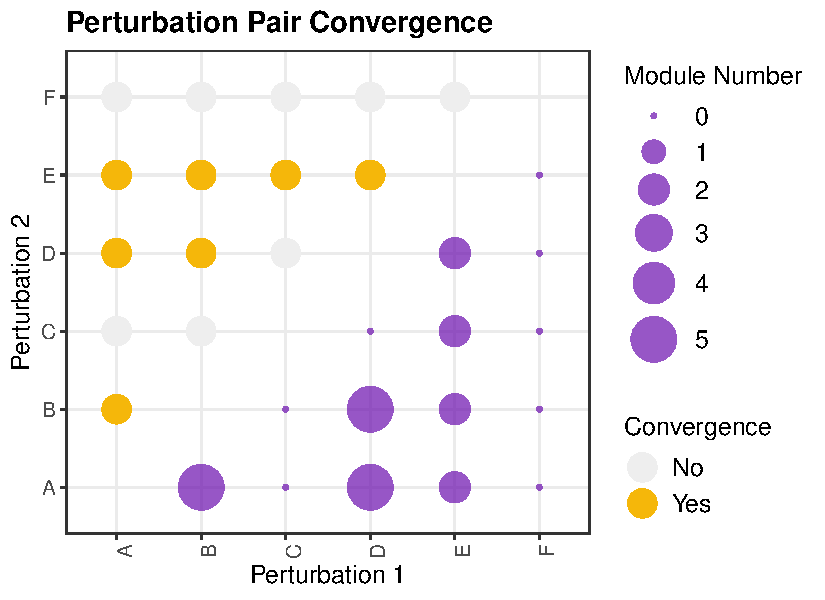
\includegraphics[width=0.6\linewidth]{paper_plot/Chen_revise.pdf}
    \caption{\textbf{Results of Dset on simulation data with perturbed gene modules.} The discovery is very to similar to that reported by XConTest in \Cref{fig: real_data_module_simu}b.} \label{Chen_revise_artificial_pert}
\end{figure}

\newpage 

\begin{figure}[tbp]
    \centering    
    \includegraphics[width=\linewidth]{paper_plot/13_splatter_pilot_combined_union.pdf}
    \caption{
    \begin{revblockr3}
    \textbf{Results of aggregated XConTest on simulation data using \textit{Splatter}.} \textbf{a.} Average log fold change of gene expression in each gene module. \textbf{b.} Testing results from aggregated XConTest. The upper half shows whether two perturbations are significantly convergent, and the lower half records the number of FSFs (i.e., detected gene modules).
    \end{revblockr3}
    }
    \label{fig: splatter_simulation}
\end{figure}

\newpage
\begin{figure}[!htbp]
  \centering
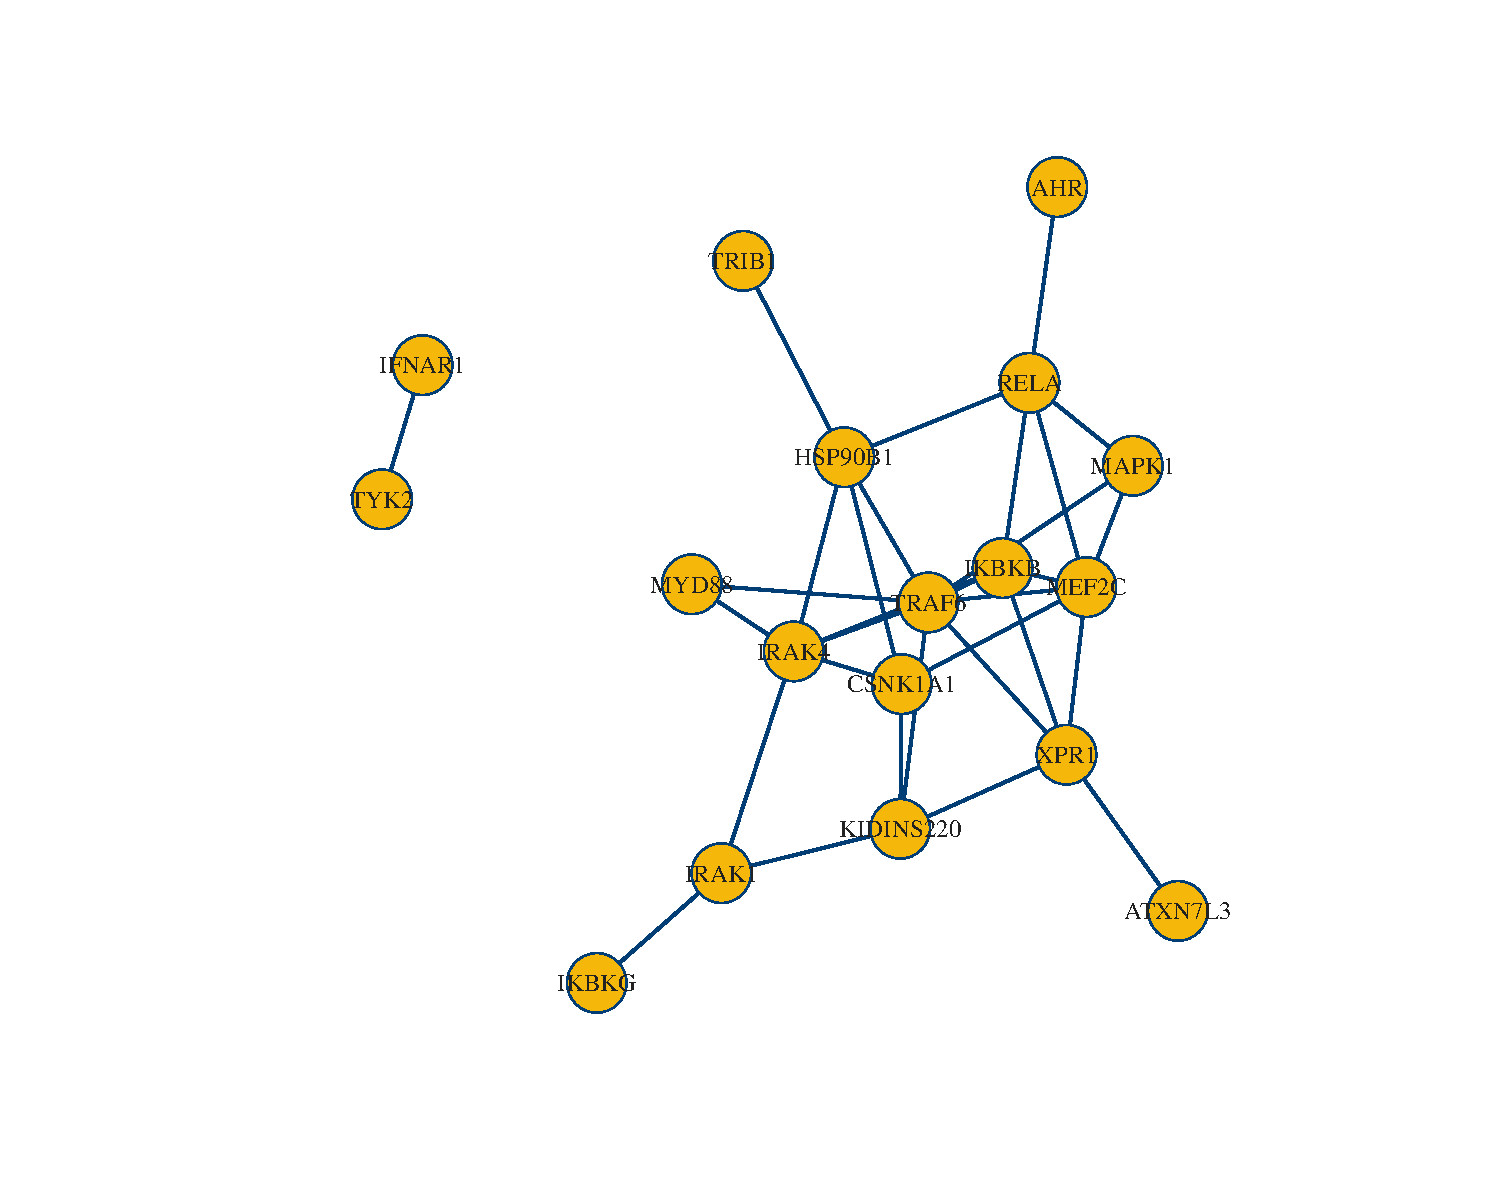
\includegraphics[width=\textwidth]{paper_plot/greater_than_3_modules.pdf}
  \caption{\textbf{Convergent perturbations with $\geq 3$ FSF-modules in the Human Macrophage Cell Line example.}}\label{fig: convergent greater than 3}
\end{figure}

\newpage
\begin{figure}[!htbp]
  \centering
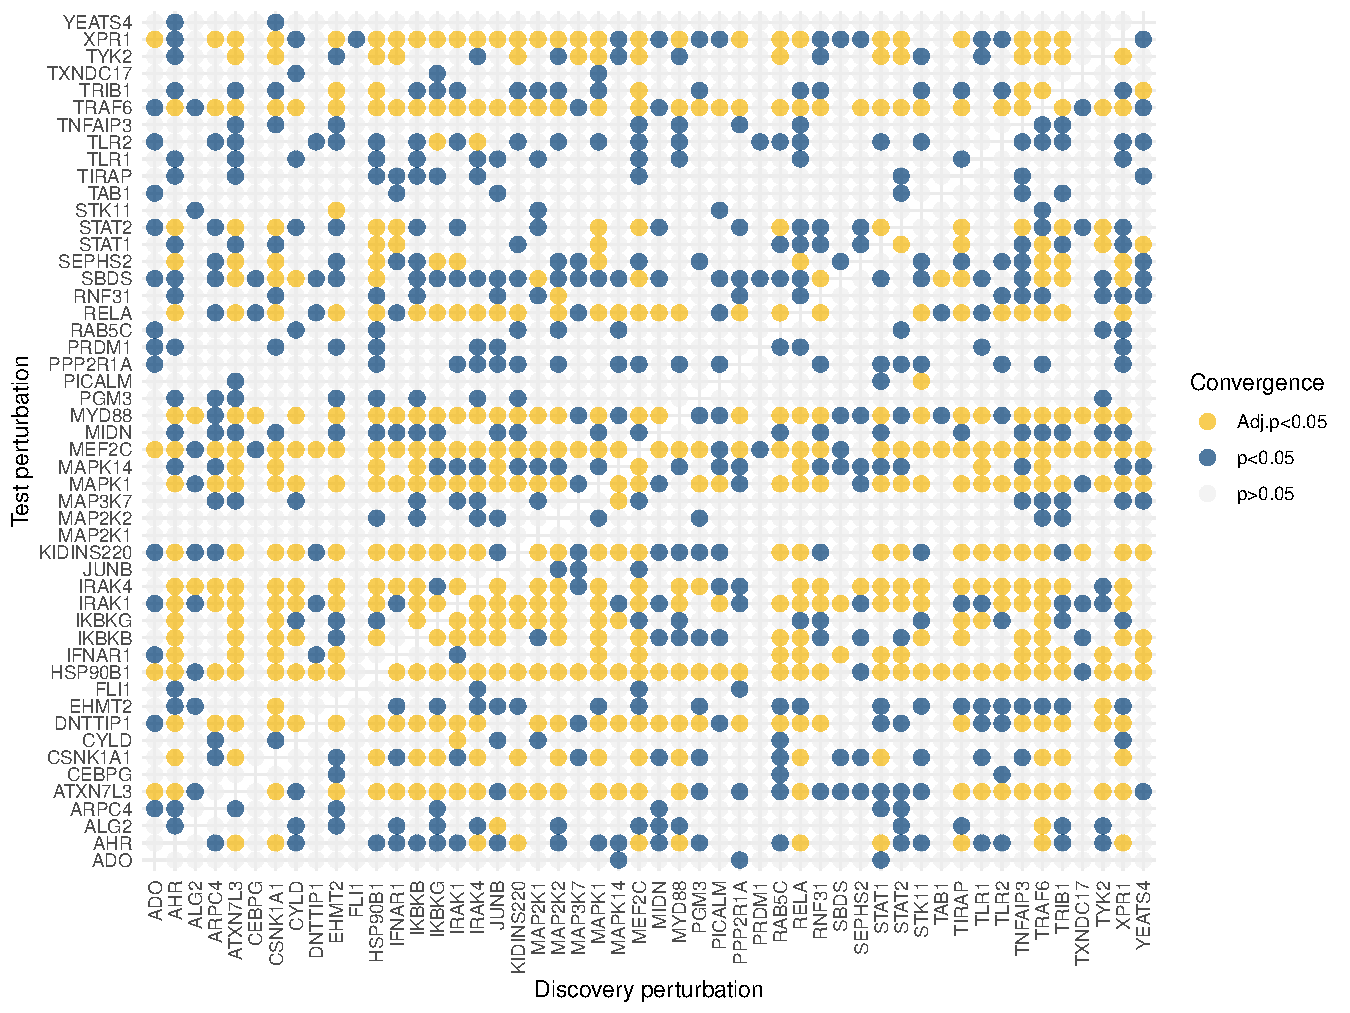
\includegraphics[width=0.7\textwidth]{paper_plot/92_51_pairwise_directional_significance.pdf}
  \caption{\textbf{Directional p-values from aggregated XConTest on the Perturb-seq experiment reported in \cite{yao2024scalable}.} Each matrix entry shows the p-value for one ordered perturbation pair. The perturbation on the x-axis is used for candidate convergence module discovery, and the perturbation on the y-axis is used for validation. Equivalently, entry $(x,y)$ reports $p_{x\to y}$. This figure displays the two directional p-values separately instead of collapsing them into $p_{\max}$ as in the main text figures.}
  \label{fig: yao directional convergence}
\end{figure}

\newpage
\begin{figure}[!htbp]
  \centering
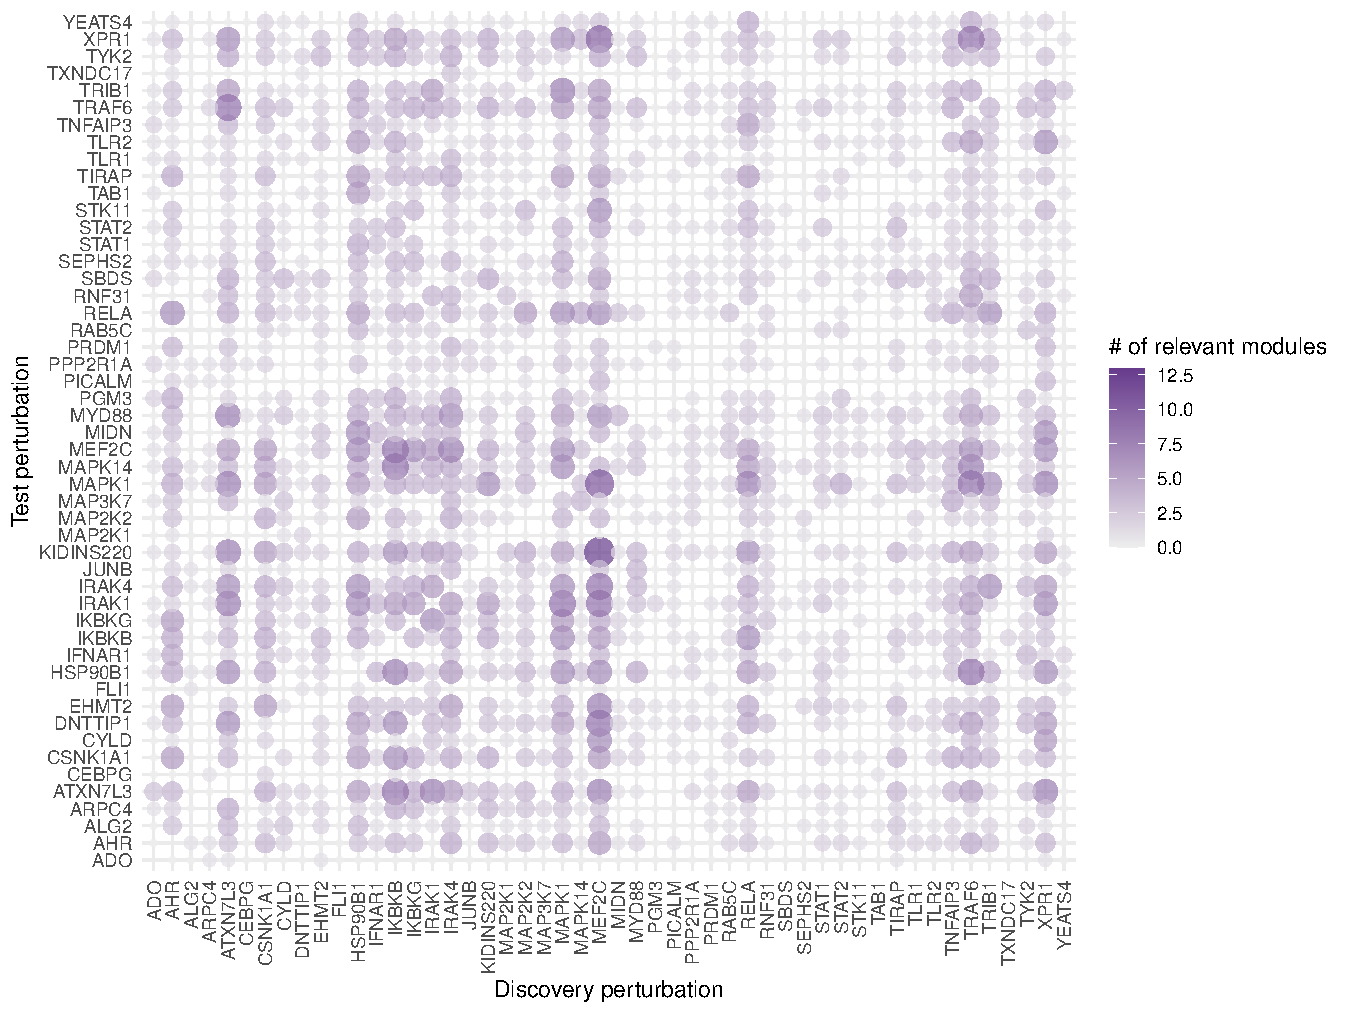
\includegraphics[width=0.7\textwidth]{paper_plot/92_51_pairwise_directional_count.pdf}
  \caption{\textbf{Directional counts of FSFs from aggregated XConTest on the Perturb-seq experiment reported in \cite{yao2024scalable}.} Each matrix entry shows the number of FSF modules for one ordered perturbation pair, where the x-axis perturbation is used for candidate module discovery and the y-axis perturbation is used for validation. One feature corresponds to one gene module in aggregated XConTest.}
  \label{fig: yao directional module counts}
\end{figure}

\newpage

\begin{table}[!tbp]
\caption{
Representative GO terms associated with selected modules. For each module, we report the biological pathway names with GO IDs. This supplementary table extends \Cref{tab: GO of modules Yao 2023} by including all modules appearing in \Cref{fig:yao_2023_main}.
}
\vspace{3mm}
\centering
\setlength{\tabcolsep}{12pt}
\renewcommand{\arraystretch}{1.3}
\label{tab:GO_of_modules_Yao_2023_selected}
\begin{tabular}{>{\raggedright\arraybackslash}p{0.15\linewidth} >{\raggedright\arraybackslash}p{0.75\linewidth}}
\toprule
\textbf{Module Index} & \textbf{Representative Gene Ontology Terms} \\
\midrule
5 & protein transport (0015031); intracellular protein transport (0006886); protein localization to membrane (0072657) \\
6 & inflammatory response (0006954); cytokine production (0001816); adaptive immune response (0002250) \\
11 & carboxylic acid metabolic process (0019752); nucleotide metabolic process (0009117); small molecule catabolic process (0044282) \\
12 & T cell activation (0042110); lymphocyte activation (0046649); antigen receptor-mediated signaling pathway (0050851); T cell receptor signaling pathway (0050852) \\
13 & cell adhesion (0007155); T cell migration (0072678); integrin-mediated signaling pathway (0007229) \\
14 & blood vessel development (0001568); skeletal system development (0001501); muscle cell differentiation (0042692) \\
17 & inorganic ion homeostasis (0098771); calcium ion homeostasis (0055074); metal ion transport (0030001) \\
20 & leukocyte migration (0050900); chemotaxis (0006935); positive regulation of T cell migration (2000406) \\
31 & response to type I interferon (0034340); defense response to virus (0051607); interferon-mediated signaling pathway (0140888); cytokine production (0001816) \\
\bottomrule
\end{tabular}
\end{table}

\newpage
\begin{figure}[tbp]
    \centering
    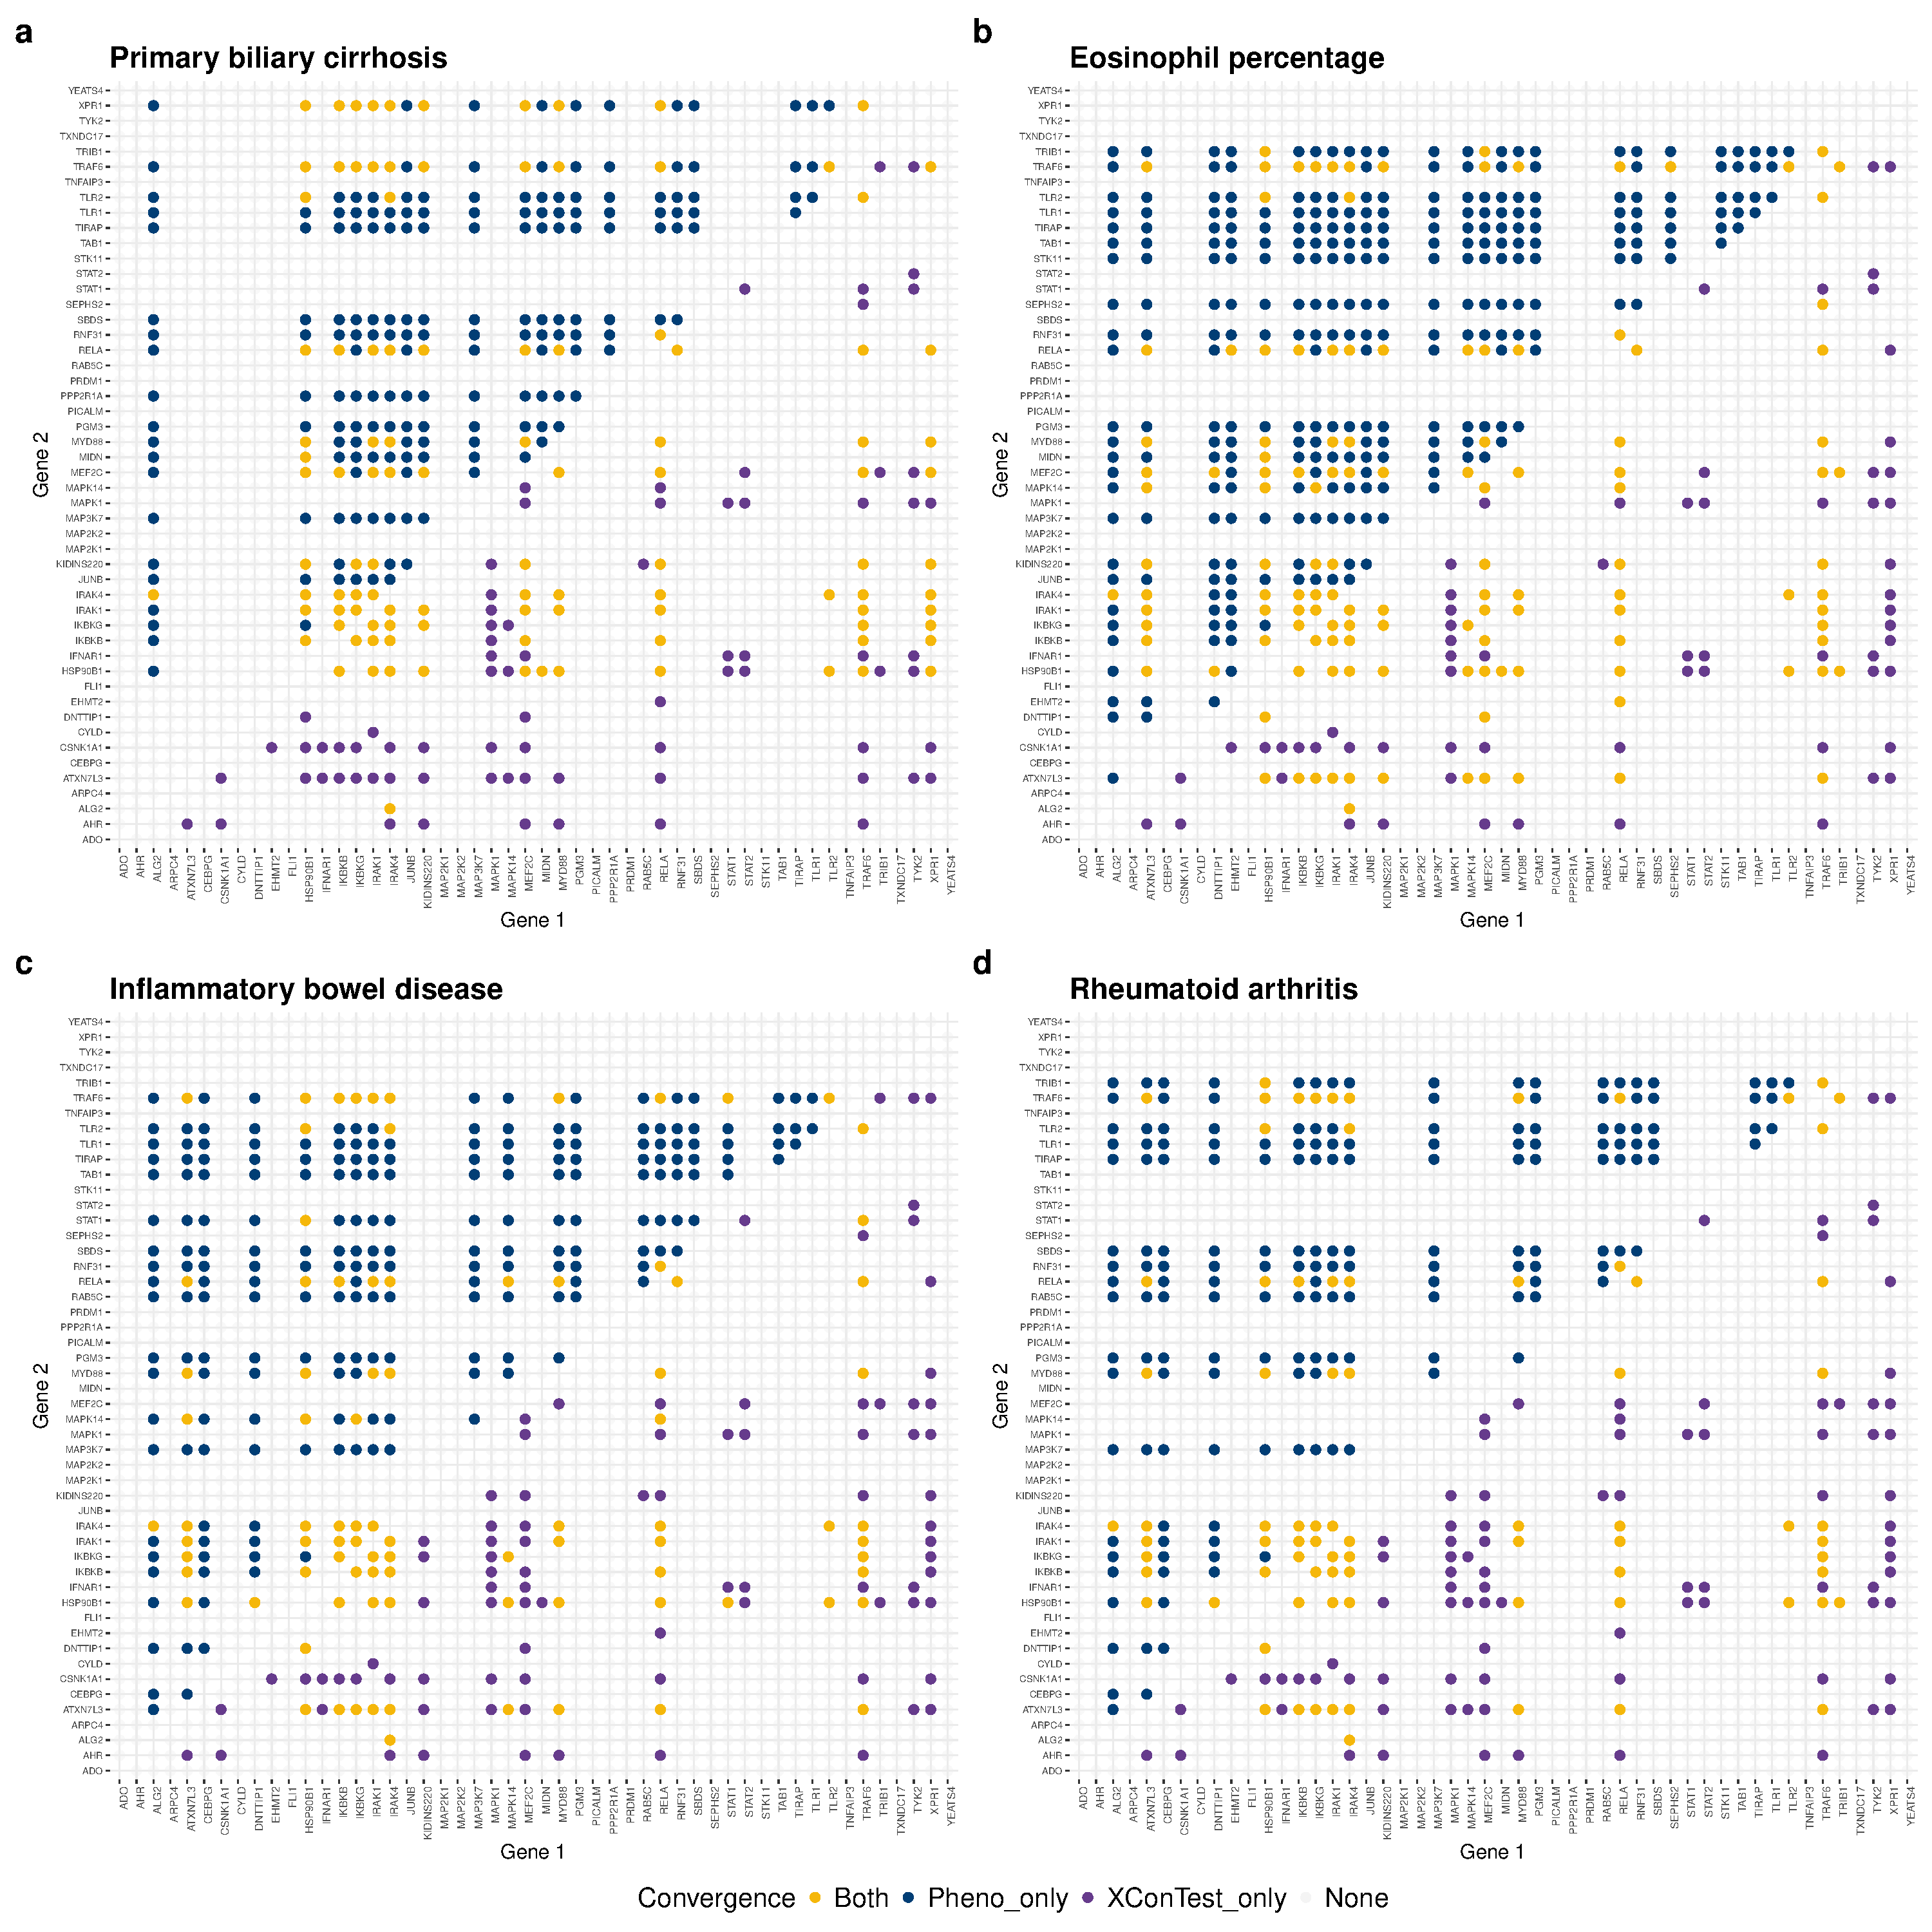
\includegraphics[width=\linewidth]{paper_plot/combined_four_3color.pdf}
    \caption{Comparison of convergence discoveries by scLinker (upper triangle) and both XConTest (lower triangle).}
    \label{fig:four_phenotypes}
\end{figure}

\newpage
\begin{figure}[tbp]
    \centering
    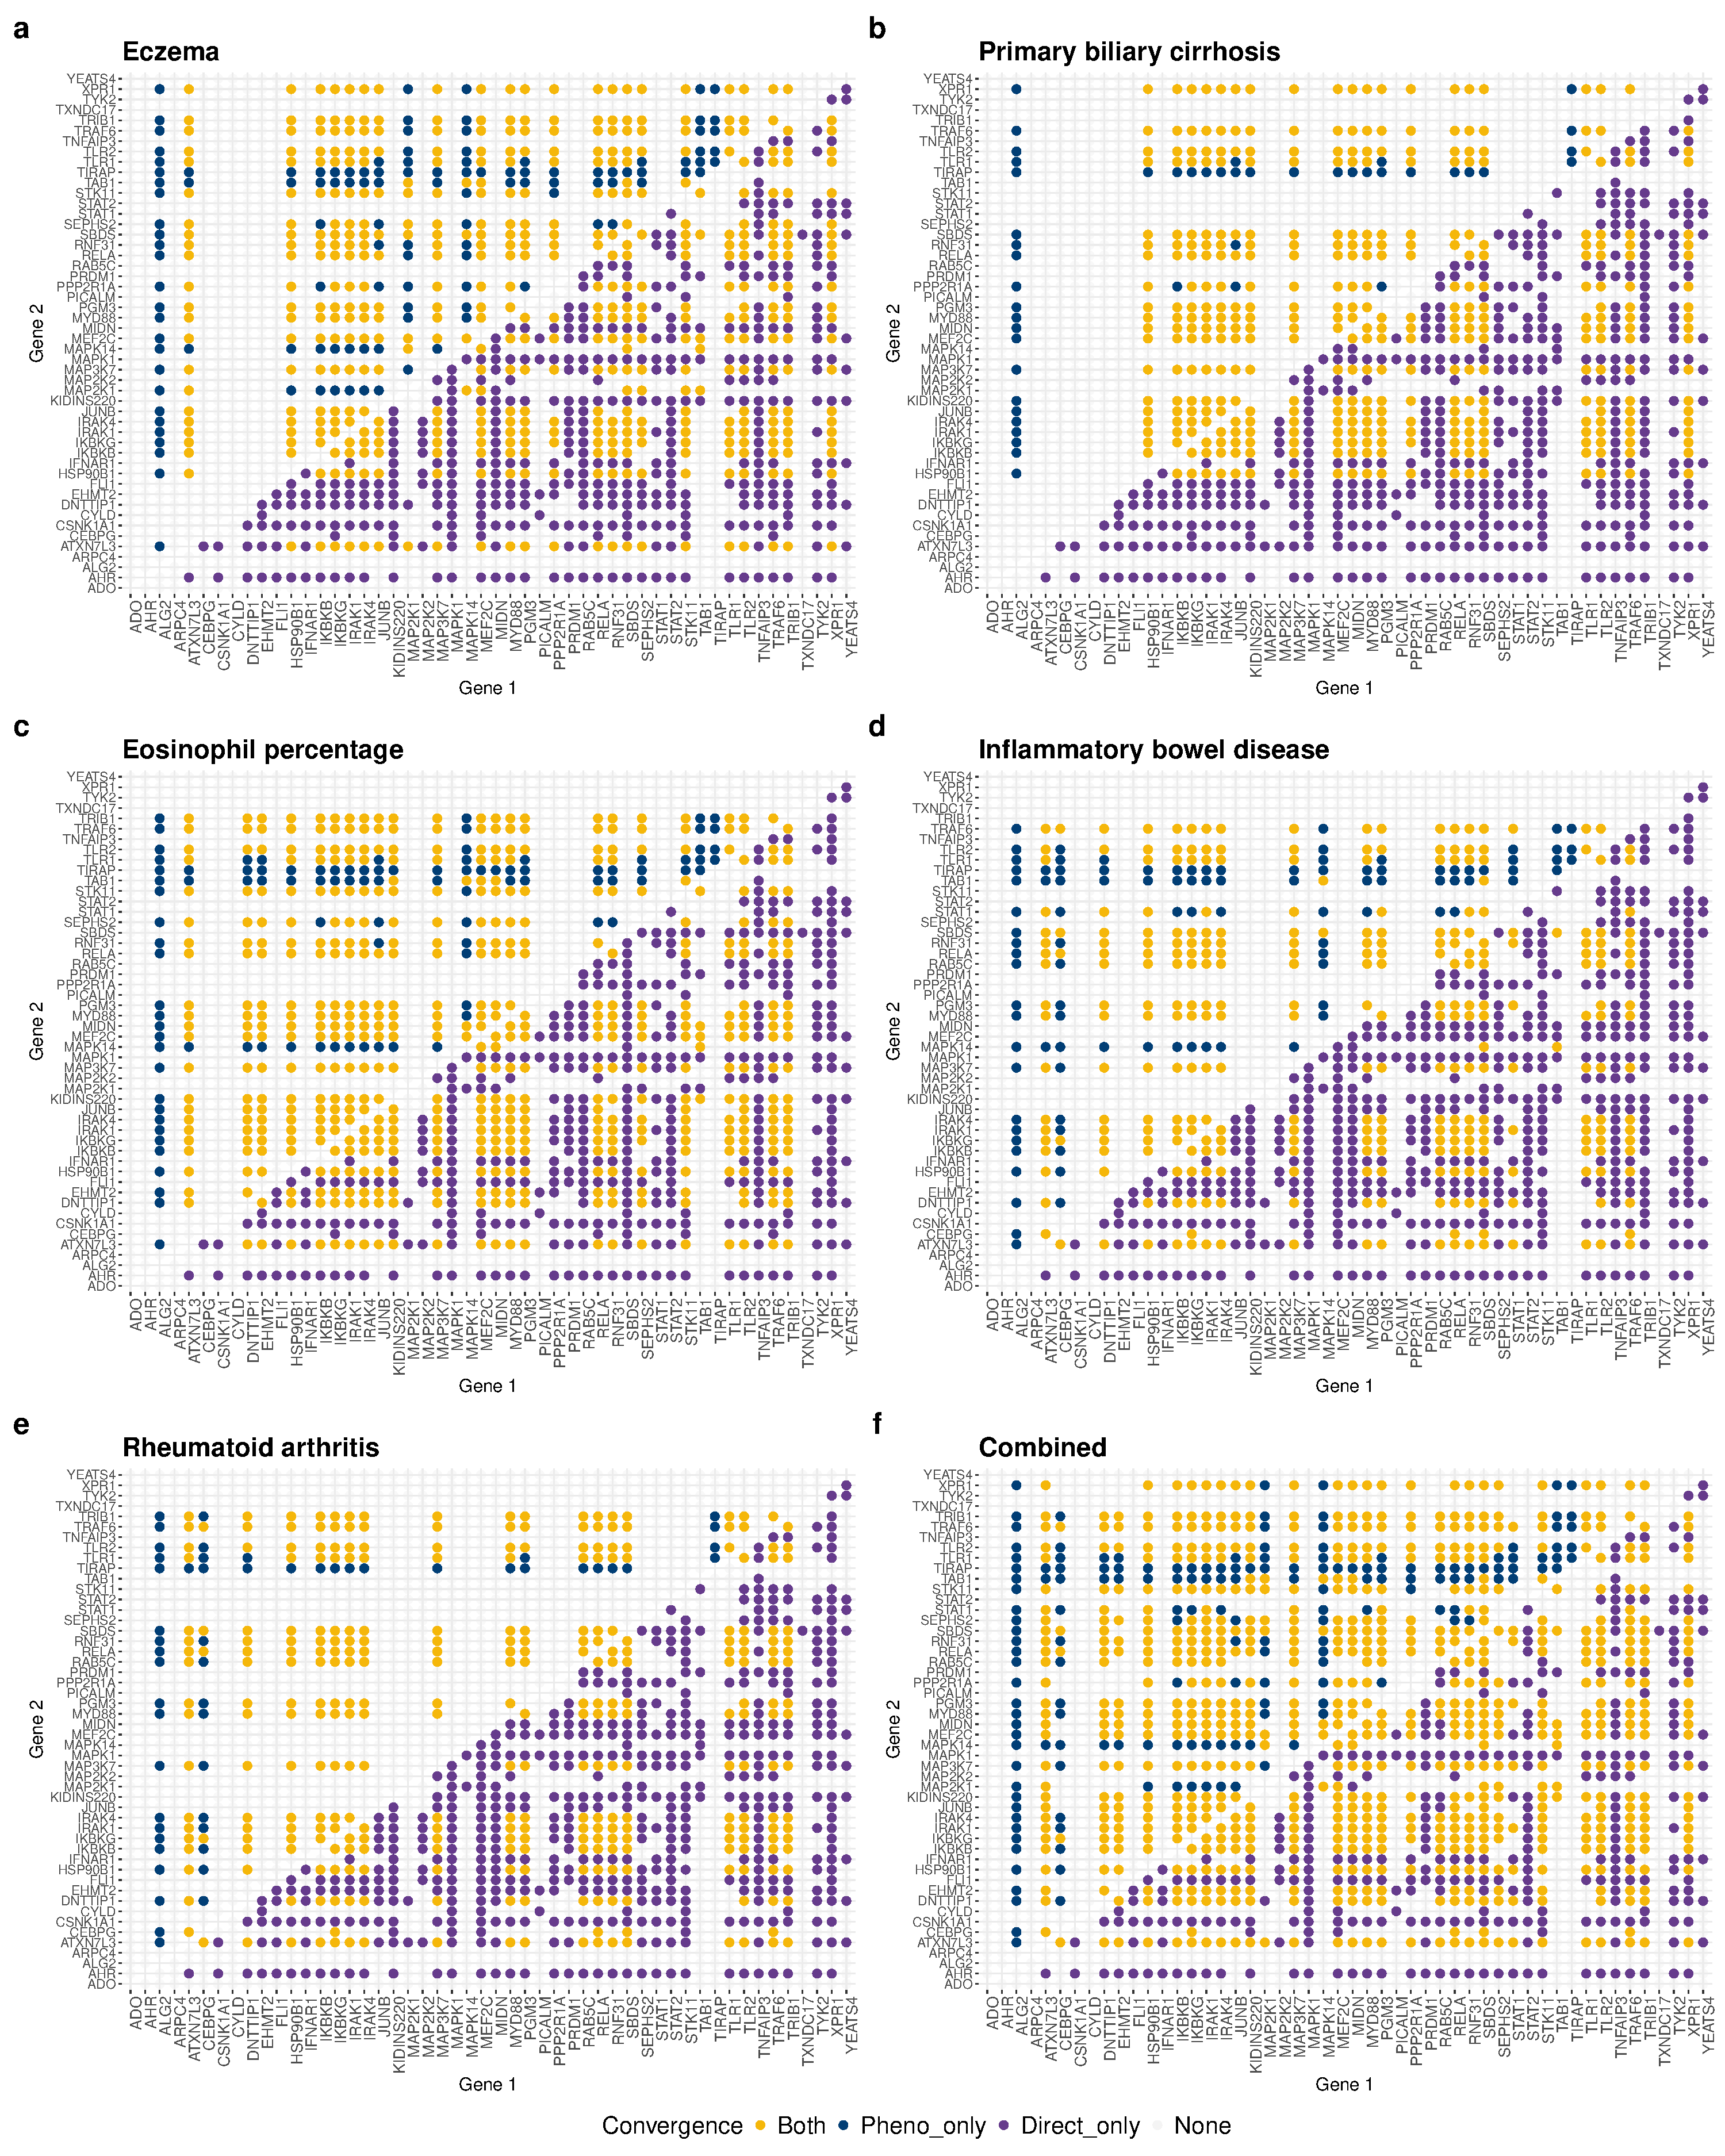
\includegraphics[width=0.9\linewidth]{paper_plot/Direct_scLinker.pdf}
    \caption{Contrast of Dset convergence with scLinker convergence for 5 phenotypes (\textbf{a}-\textbf{e}) and at least one phenotype \textbf{f}.}
    \label{fig:DirectscLinker}
\end{figure}

\newpage
\begin{figure}[tbp]
    \centering
    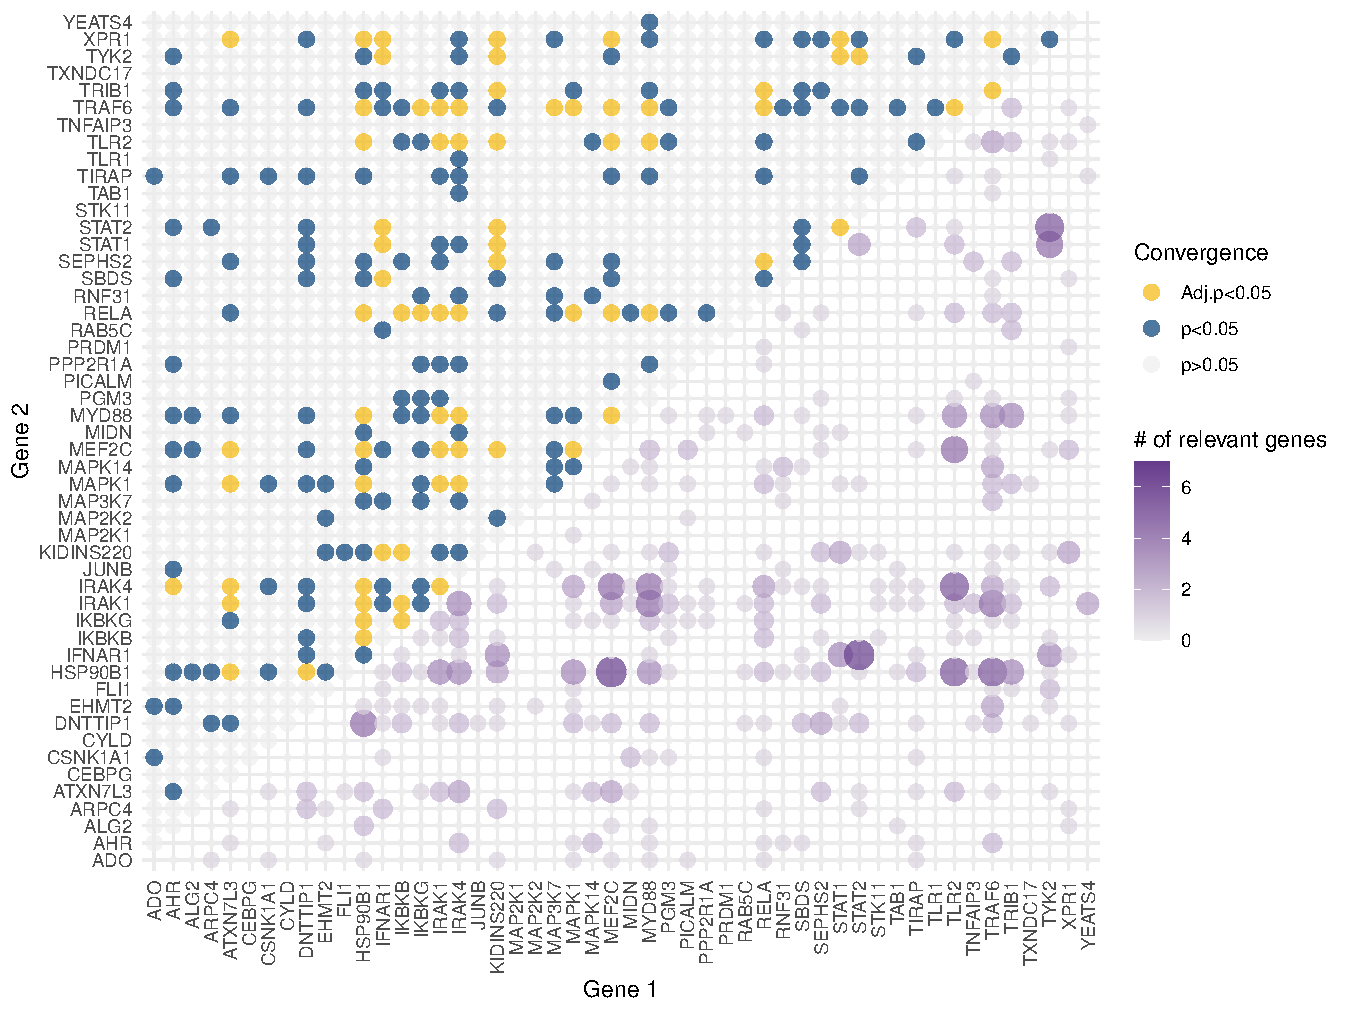
\includegraphics[width=0.9\linewidth]{paper_plot/G3_G1_pairwise_overall_significance.pdf}
    \caption{\textbf{Sensitivity analysis of the Perturb-seq experiment reported in \cite{yao2024scalable}}.
    The experiment is similar to that reported in \Cref{fig:yao_2023_main}a, instead of using 2000 top-expressed genes, we trim the list further down to immunity-related gene modules---labeled as module 6, 12, 13, 20 and 31 in \Cref{tab:GO_of_modules_Yao_2023_selected}. In total, there are 201 genes used in this analysis. Gene-wise XConTest is applied instead of the aggregated XConTest to establish a more stringent convergence (the perturbations need to induce strong changes in the same gene). Note that the special STAT1-STAT2-TYK2 cluster (\Cref{fig:yao_2023_main}f) still establishes the strongest convergence signal. The discovery in the MYD88 pathway (\Cref{fig:disease_mechanism_convergence}c) is also preserved.}
    \label{fig: sensitivity_analysis}
\end{figure}

\end{document}
